%!TEX root = main.tex


\documentclass[11pt,a4paper]{article}
\usepackage{acl2015}
\usepackage{times}
\usepackage{url}
\usepackage{latexsym}
\usepackage{tabularx}

\usepackage{graphicx} % support the \includegraphics command and options
\usepackage{rotating}

\usepackage[normalem]{ulem}

\usepackage{xspace}
\usepackage{xcolor}
\usepackage{booktabs}
\newcommand{\Eye}{Eye-tracking\xspace}
\newcommand{\eye}{eye-tracking\xspace}
\newcommand{\mono}{\nobreak{\emph{monolingual}}\xspace}
\newcommand{\bil}{\nobreak{\emph{bilingual}}\xspace}
\newcommand{\monos}{\nobreak{\emph{monolinguals}}\xspace}
\newcommand{\bils}{\nobreak{\emph{bilinguals}}\xspace}
\newcommand{\src}{\nobreak{\emph{source-only}}\xspace}
\newcommand{\srctgt}{\nobreak{\emph{source+target}}\xspace}
\newcommand{\tgt}{\nobreak{\emph{target-only}}\xspace}
\newcommand{\lshort}{\nobreak{\emph{short}}\xspace}
\newcommand{\lmid}{\nobreak{\emph{medium}}\xspace}
\newcommand{\llong}{\nobreak{\emph{long}}\xspace}
\newcommand{\gamet}{\nobreak{\emph{scenario}}\xspace}
\newcommand{\gamets}{\nobreak{\emph{scenarios}}\xspace}

\newcommand{\qmin}{\nobreak{\emph{worst}}\xspace}
\newcommand{\qmax}{\nobreak{\emph{best}}\xspace}
%\newcommand{\omitted}{\nobreak{https://github.com/Qatar-Computing-Research-Institute/iAppraise}\xspace}
\newcommand{\paco}[1]{{\color{blue}[FG]:#1}}
\newcommand{\ahmed}[1]{{\color{brown}[A$^3$]:#1}}
\newcommand{\irina}[1]{{\color{violet}[IT]:#1}}
\newcommand{\hassan}[1]{{\color{green}[HS]:#1}}
\newcommand{\stephan}[1]{{\color{gray}[SV]:#1}}
\newcommand{\alert}[1]{{\color{note}[!!!!]:#1}}

%%% MT metrics and variants
\newcommand{\qcri}{\nobreak{DR}}
\newcommand{\qcril}{\nobreak{DR-{\sc lex}}}
\newcommand{\drLEXe}{\nobreak{DR-{\sc lex}$_e$}}
\newcommand{\sqcri}{\nobreak{\sc dr}}
\newcommand{\sqcril}{\nobreak{\sc dr-{\scriptsize lex}}}
\newcommand{\full}{\nobreak{\emph{full}}}
\newcommand{\nor}{\nobreak{\emph{no\_rel}}}
\newcommand{\non}{\nobreak{\emph{no\_nuc}}}
\newcommand{\nonr}{\nobreak{\emph{no\_nuc \& no\_rel}}}
\newcommand{\nostr}{\nobreak{\emph{no\_discourse}}}

\newcommand{\dummy}{\nobreak{\emph{dummy}\hspace{3pt}}}

% DR-based individual metrics
\newcommand{\drLEX}{\nobreak{DR-{\sc lex}$_{1}$}}
\newcommand{\dr}{\nobreak{DR-{\sc nolex}}}
\newcommand{\drLEXto}{\nobreak{DR-{\sc lex}$_{2}$}}
\newcommand{\drLEXoo}{\nobreak{DR-{\sc lex}$_{1.1}$}}
\newcommand{\drLEXot}{\nobreak{DR-{\sc lex}$_{1.2}$}}
%\newcommand{\drLEXtt}{\nobreak{DR-{\sc lex}$_{2.1}$}}

% DiscoTK metrics
\newcommand{\disco}{\nobreak{DiscoTK}}
\newcommand{\discolight}{\nobreak{{\sc DiscoTK}$_{light}$}}
\newcommand{\discoparty}{\nobreak{{\sc DiscoTK}$_{party}$}}
%

%\newcommand{\sqcri}{\nobreak{\sc dr}}
%\newcommand{\sqcril}{\nobreak{\sc dr-{}$}}
%
\newcommand{\spede}{\nobreak{\sc spede07pP}}
\newcommand{\sempos}{\nobreak{SEMPOS}}
\newcommand{\amber}{\nobreak{AMBER}}
\newcommand{\meteor}{\nobreak{\sc Meteor}}
\newcommand{\terrorcat}{\nobreak{\sc TerrorCat}}
\newcommand{\simpbleu}{\nobreak{SIMPBLEU}}
\newcommand{\ter}{\nobreak{TER}}
\newcommand{\bleu}{\nobreak{BLEU}}
\newcommand{\posf}{\nobreak{\sc posF}}
\newcommand{\block}{\nobreak{\sc BlockErrCats}}
\newcommand{\sblock}{\nobreak{\sc BEC}}
\newcommand{\word}{\nobreak{\sc WordBlockEC}}
\newcommand{\sword}{\nobreak{\sc WBEC}}
\newcommand{\xen}{\nobreak{\sc XEnErrCats}}
\newcommand{\sxen}{\nobreak{\sc XEEC}}
\newcommand{\sagan}{\nobreak{\sc SAGAN-STS}}
%%%
\newcommand{\nist}{\nobreak{NIST}}
\newcommand{\rouge}{\nobreak{\sc Rouge}}
%%%
\newcommand{\asiyaall}{\nobreak{Asiya-{\sc all}}}
\newcommand{\asiyaix}{\nobreak{Asiya-{\sc 0809}}}
\newcommand{\lex}{\nobreak{Asiya-{\sc lex}}}
\newcommand{\syn}{\nobreak{Asiya-{\sc syn}}}
\newcommand{\srl}{\nobreak{Asiya-{\sc srl}}}
\newcommand{\dis}{\nobreak{Asiya-{\sc sem}}}

%%% tools
\newcommand{\asiya}{\nobreak{\sc Asiya}}

%%% language pairs
\newcommand{\csen}{\nobreak{\sc cs-en}}
\newcommand{\deen}{\nobreak{\sc de-en}}
\newcommand{\esen}{\nobreak{\sc es-en}}
\newcommand{\fren}{\nobreak{\sc fr-en}}
\newcommand{\ruen}{\nobreak{\sc fr-en}}

%%% corpora
\newcommand{\wmt}{\nobreak{\sc wmt}}
\newcommand{\wmte}{\nobreak{\sc wmt11}}
\newcommand{\wmtt}{\nobreak{\sc wmt12}}
\newcommand{\wmth}{\nobreak{\sc wmt13}}
\newcommand{\wmtf}{\nobreak{\sc wmt14}}

%%% inline lists
\newcommand{\Ni}{({\em i})~}
\newcommand{\Nii}{({\em ii})~}
\newcommand{\Niii}{({\em iii})~}
\newcommand{\Niv}{({\em iv})~}
\newcommand{\Nv}{({\em v})~}
\newcommand{\Na}{({\em a})~}
\newcommand{\Nb}{({\em b})~}
\newcommand{\Nc}{({\em c})~}

%\setlength\titlebox{5cm}

% You can expand the titlebox if you need extra space
% to show all the authors. Please do not make the titlebox
% smaller than 5cm (the original size); we will check this
% in the camera-ready version and ask you to change it back.


\title{How do Humans Evaluate Machine Translation}

\author{Francisco Guzm\'an\hspace*{1.5mm}
Ahmed Abdelali\hspace*{1.5mm}
Irina Temnikova\hspace*{1.5mm}
Hassan Sajjad\hspace*{1.5mm}
\hbox{\rm and}\hspace*{1.5mm}Stephan Vogel\\
ALT Research Group\\
Qatar Computing Research Institute, HBKU\\
%, Qatar Foundation\\
{\tt\{fguzman,aabdelali,itemnikova,hsajjad,svogel\}@qf.org.qa}}

\date{}

\begin{document}
\maketitle
\begin{abstract}
In this paper, we take a closer look at the MT evaluation process from a \emph{glass-box} perspective using \eye. We analyze two aspects of the evaluation task -- the background of evaluators (\emph{monolingual or bilingual}) and the sources of information available, and we evaluate them using time  and consistency as criteria. % the factor of time and consistency. 
Our findings show that \monos are slower but more consistent than \bils, especially when only target language information is available. 
When exposed to various sources of information, evaluators in general take more time and in the case of \monos, there is a drop in consistency.  Our findings suggest that to have consistent and cost effective MT evaluations, it is better to use \monos with only target language information.  

\end{abstract}

\section{Introduction}
%!TEX root = main.tex

%There are several alternatives to perform human evaluation of Machine Translation. 
Each year thousands of human judgments are used to evaluate the quality of Machine Translation (MT) systems to determine %and decide 
which algorithms and techniques are to be considered the new state-of-the-art. 
%\hassan{I did not like the second part of pervious sentence after "and decide". we may remove it.}
In a typical scenario 
%for human evaluation of Machine Translation (MT),
 human judges evaluate a system's output (or \emph{hypothesis}) by comparing it to a source sentence and/or to a reference translation. Then, they score the hypothesis according to a set of defined criteria such as \emph{fluency} and \emph{adequacy} \cite{white1994}; or rank a set of hypotheses in order of preference \cite{vilar-EtAl:2007:WMT,callisonburch-EtAl:2007:WMT}.

Evaluating MT output can be a challenging task for a number of reasons: it is tedious and therefore evaluators can lose interest quickly; it is complex, especially if the guidelines are not well defined; and evaluators can have difficulty distinguishing between different aspects of the translations \cite{callisonburch-EtAl:2007:WMT}. \\
%Furthermore, it can be highly subjective as evaluators develop their own \emph{intrinsic} rules of thumb to evaluate translations. 
As a result, evaluations suffer from low inter- and intra-annotator agreements \cite{Turian2003,Snover06astudy}. Yet, as \newcite{Sanders2011} argue, using human judgments is essential to the progress of MT because: \Ni automatic translations are produced for a human audience; and \Nii human understanding of the \emph{real} world allows to assess the importance of the errors made by MT systems.

Most of the research in human evaluation has focused on analyzing the criteria to use for evaluation, and has regarded the evaluation process as a \emph{black-box}, where the inputs are different sources of information (i.e source text, reference translation, and translation hypotheses), and the output is a score (or preference ranking).

In this paper, we focus on analyzing evaluation from a different perspective. First, we regard the process as a \emph{glass-box} and use \eye to monitor the times evaluators spend digesting different sources of information (\emph{scenarios}) before making a judgment. Secondly, we contrast how the availability of such sources can affect the outcome of the evaluation. Finally, we analyze how the background of the evaluators (in this case whether they are \emph{monolingual} or \emph{bilingual}) has an effect on the consistency and speed in which translations are evaluated. Our main research questions are:

\begin{itemize}
%\setlength{\itemindent}{-.1in}
\item Given different \gamets, what source of information do evaluators use to evaluate a translation? Do they use the source text, the target text, or both? Does the availability of specific information changes the consistency of the evaluation?
%\item Do they follow a specific order of areas of interest while evaluating? 
%How long do they spend in each area? %and %\sout{in general} 
%overall to give an evaluation score?
%\sout{to a translation}?
%\end{itemize}

% OLD one:
% \item Given the current layout, what kind of information do evaluators use to decide on the score of a translation.
%-- Do they use the source information, the target information, or both?
%-- For how long do they score?
%-- Is there a specific order in which users evaluate?

\item Are there differences of behavior between \emph{bilinguals} (i.e. evaluators fluent in both source and target languages) and \emph{monolinguals} (i.e. evaluators fluent only in the target language)?
Which group is more consistent?

%\item Are there differences in behavior when evaluating \emph{good} vs. \emph{bad} translations?

\end{itemize}

Our goal is to provide actionable insights that can help to improve the process of evaluation, especially in large-scale shared-tasks such as WMT. In the next sections we summarize related work, provide details of our experimental setup, and analyze and discuss the results of our experiment. 
%The remainder of this paper is divided as follows: First, we give a survey for related work and then we detail the method used in setting our experiments followed by results. Finally, we provide discussions for our findings and a conclusion.


\vspace{5pt}
\section{Related Work}
\vspace{5pt}
%!TEX root = main.tex

% Irina's notes: merge somehow:
%A large variety of automatic metrics, semi-automatic (or human-in-the-loop) and human judgements for machine translation evaluation exist \cite{Dorr2011}.
%Although human judgements have a number of limitations, and are trying to be replaced by automatic, or semi-automatic metrics, they continue to be used mostly due to the fact that translations are produced for human readers. \cite{Dorr2011}.
%Two kinds of human judgements are mostly taken into account: MT output \emph{fluency} and \emph{adequacy}. While \emph{fluency} requires that a speaker fluent in the target language reads the MT output and determines whether it is fluent, \emph{adequacy} requires that a speaker fluent both in the source language and in the target language determines whether all the meaning of the source text has been transferred to the target language \cite{Dorr2011}. 
%The limitations of human judgements include: difficulty to find evaluators, high cost; lack of repeatability; slowness of evaluation; subjectivity; evaluators' opinions influenceable by their knowledge of the topic of the text; by their experience as translators/evaluators; by their familiarity with the system layout; etc.
%In addition to that there were already several attempts to discuss the necessity of having bilingual evaluators. As they need to speak both the source and the target language fluently, they are more difficult, as well as more expensive to recruit than monolingual evaluators. For the moment, the use of bilingual evaluators is still considered as gold standard \cite{Dorr2011}. While monolingual evaluators are sometimes used for MT evaluation when supplied with reference translations \cite{Dorr2011}.
%In this paper, we focus in analyzing different aspect of the process of MT human evaluation using \eye information.

Previous work on human evaluation has focused on various aspects of the evaluation process ranging from 
categorization of the possible scenarios \cite{Sanders2011} to the effectiveness of the evaluation criteria \cite{callisonburch-EtAl:2007:WMT}. 
%
%In the past, researchers have proposed different methods to assess the quality of a translation, such as the direct evaluation of \emph{adequacy} and \emph{fluency}, and the ranking-based evaluation \cite{vilar-EtAl:2007:WMT,callisonburch-EtAl:2007:WMT}. Unfortunately, humans have a hard time assigning an absolute score to a translation, and in major MT evaluations, absolute scores were phased out in favor of ranking-based evaluations or task-based evaluations (e.g. HTER). It has been shown that using such ranking-based assessments yields much higher inter-annotator agreement \cite{callisonburch-EtAl:2007:WMT}. 
%
\newcite{callisonburch-EtAl:2007:WMT} define several criteria to evaluate the effectiveness of a MT evaluation task:
\Ni The \emph{ease} with which humans are able to perform the task; \Nii the \emph{agreement} with respect to other annotators; and \Niii the \emph{speed} with which annotations can be collected. %They assessed three different ways of evaluating sentences:

%\newcite{callisonburch-EtAl:2007:WMT} 

Based on those criteria they recommended that evaluations should be done in the form of ranking translations against each other  instead of assigning absolute scores to individual translation because ranking is easier to perform, can be done faster, and produces evaluations with higher levels of inter-annotator agreement. 
%Yet, no specific criteria to consider when evaluating a translation were provided. 
%, and annotators have different criteria of what makes a \emph{good} or a \emph{bad} translation.  
%Instead, 
%Furthermore, 
As a result, recent WMT evaluations have adopted this evaluation-by-ranking approach and instructions are \emph{kept minimal} by only asking the evaluator to rank hypotheses from worst to best \cite{Bojar2011}.

%However, even in ranking-based tasks, annotators have different criteria of what makes a \emph{good} or a \emph{bad} translation. 
%This is often determined by their background or level of experience and can determine the performance of an evaluator, as well as undermine the quality of the evaluation.
%

%1. Assigning scores according to a five-point scale for adequacy and fluency. % following the guidelines described in \cite{LDC2005},
%2. Ranking hypotheses relative to other's. %quality from best to worst.
%3. Ranking the translations of selected \emph{syntactic constituents} drawn from the source sentence.
%
%According to \new/cite{callisonburch-EtAl:2007:WMT}, there are several criteria that define the MT evaluation task:
%\Ni The \emph{ease} with which humans are able to perform the task; \Nii the agreement w.r.t. other annotators, and the \emph{speed} with which annotations can be collected.
%
%In their observations, people had a hard time distinguishing between the \emph{fluency} and \emph{adequacy} aspects of a translation, and found that there is a high correlation between both scores. Furthermore, the lack of clear guidelines further complicates the assessment (e.g. how is \emph{meaning} quantified, how do grammatical errors affect different levels of fluency). Therefore, \newcite{callisonburch-EtAl:2007:WMT} point out that each annotator develops their own rules of thumb.
%By asking annotators to rank the hypotheses, the task was simplified considerably, and inter-annotator agreement increased. Furthermore, when asked to rank only constituents, additional improvements were observed.
%In terms of time, ranking constituents reduced the evaluation time to about 11 seconds on average, when compared to 26 seconds on average for the full hypothesis. Note however, that the times were not normalized by the number of words in the hypothesis/constituent. In summary, 

In this work, we consider the three criteria proposed by \newcite{callisonburch-EtAl:2007:WMT}: \emph{ease}, \emph{agreement} and \emph{speed}; but with a few differences. Regarding \emph{ease}, instructions are kept minimal, and the evaluation criteria is left to the evaluator to decide (or discover). Furthermore, by framing the evaluation as a game we aim to keep participants engaged, and make the evaluation task easier. %,  and providing feedback on their performance based on other human annotations.
With respect to the other two criteria, we use them to analyze two different aspects of the evaluation process: the sources of information available to the evaluator, and the background of the evaluator. 

%as much as possible we add \eye to human evaluation and analyze the criteria defined by \newcite{callisonburch-EtAl:2007:WMT} (ease, agreement and speed). The motivation behind using \eye to extract information about how users conduct evaluation is helping to better understand the process and therefore allow to %We design the evaluation process in a way that 
%improves evaluators engagement and reduce the bias in the process of evaluating a translation.
%compares various type of evaluators (monolingual, bilingual) w.r.t different information scenarios. We show that \eye helps to .... \hassan{a few words from discussion}  
%Currently, there the standard mode of operation is...

% However, we rarely question our assumptions about the task.


%\paco{The motivation behind using eye-tracking to extract information on how users evaluate a translation. Intuitively, we would like to use that information to reduce the bias in the process of evaluating a translation.}

%As mentioned before, there are two main challenges when presenting an evaluation task: \Ni how to make the task \emph{less} tedious, i.e. increasing engagement, to preserve the user's focus;  and \Nii how to develop consistent guidelines to increase inter-annotator agreement. For \Ni, \cite{doherty2010eye} proposed to have a comprehension questionnaire aimed to encourage the user's focus retention, while for \Nii, ranking tasks have been proposed. 
%Instead, here we propose a evaluation as a game, in which users have to build their own strategies to mimic the evaluation of an \emph{expert} translator. This serves to both purposes: to keep the users engaged by immediately given feedback after each evaluation; and to train users to develop consistent strategies that mimic a \emph{gold standard}.

Eye-tracking has been previously used in MT evaluation research for different purposes. 
%
%
%~\cite{stymne2012eye,carl2012translog,alabau2014casmacat,doherty2014assessing,doherty2010eye}. 
% The work of \cite{doherty2010eye}, Stymne et al.~\shortcite{stymne2012eye}, and Doherty and O'Brien~\shortcite{doherty2014assessing} are most relevant to us.
%
%
\newcite{doherty2010eye} used \eye to
%the Tobii 1750 eye-tracker. 10 native speakers of French were asked to read and 
%
evaluate the comprehensibility of machine translation output in French, by asking native speakers to read MT output. 
%
%of French. 
% to read previously evaluated by human evaluators 25 well-translated sentences and 25 poorly translated sentences.
%50 sentences, translated by an automatic machine translation system into French. 25 of the sentences were rated as excellent in previous human rating, and 25 - as poor. 
%Four eye-tracking variables were used: 1) gaze time; 2) fixations count; 3) pupil dilation; and 4) average fixation duration. 
%
%
They found that eye-tracking data 
%(specifically gaze time and fixation count)
had a slight correlation with HTER scores. 

\newcite{stymne2012eye} applied eye-tracking to machine translation error analysis. 
%
%
%33 university students were asked to read the text outputs of three machine translation systems, along with a human-produced text, and evaluate the text quality. 
%Eye-tracking was recorded using SMI Remote Eye iView, and the following variables were recorded: 1) average gaze time and 2) fixations count. 
%
%
They found that longer gaze time and and a higher number of fixations correlate with high number of errors in the MT output. 
%
% rather than on correct parts, as well as differences in eye-tracking data for different types of MT errors. The study concluded that eye-tracking could be used as a complementary information to MT error analysis.
Doherty and O'Brien~\shortcite{doherty2014assessing} used eye-tracking to evaluate the quality of raw machine translation output in terms of its \emph{usability} by an end user. 
%
%
%In order to achieve this, an online service documentation was translated using Google Translate, and 30 participants were asked to read the documentation. 
%, and perform tasks, based on this documentation. An eye-tracking tool, Tobii 1750, was used to record the eye-movements of the participants while reading the documentation and executing the tasks in order to measure the cognitive effort involved in processing the documentation. The following eye-tracking variables were used: 1) fixations count; and 2) average fixation duration. 
%
%
They concluded that eye-tracking correlates well with the other measures which they used for their study. 
In this work, we use \eye to observe which sources of information evaluators use while performing an MT evaluation task and how this impacts the task completion time and the consistency in their judgements.
 
%We use this information to learn where do evaluators look.
%None of the previous work described the eye moving behavior of people performing the machine translation evaluation task. 





\section{Method}
%!Tex root = main.tex
In order to understand how humans evaluate MT, we ran an evaluation experiment using \eye, involving $20$ human participants, half of them \mono in English and the other half \bil in Spanish-English. We chose the Spanish-English language pair because of the large amount of freely available data (e.g. WMT) and the sizable pool of available participants in our environment. In our setup, we contrasted the evaluation procedure under alternative \gamets in which different sources of information (e.g. source sentence, reference translation) are available.  To keep things simple, we only asked participants to evaluate one translation at a time and provide a single score representing the translation quality. To prevent biasing the behavior of the participants, and to encourage them to evaluate translations \emph{naturally}, participants were not given any precise instructions regarding the requirements of a \emph{good} translation. To increase engagement, we formulated the evaluation experiment as a game, where participants are provided feedback after each evaluation according to how close their own score was to a precomputed quality score. Below, we further describe the data used, the different \gamets, the background of the participants, and other details of our experiment. %participants read different combinations of translation evaluation data using the open-source MT evaluation platform Appraise ~\cite{federmann2012appraise} and give an evaluation score, while an eye-tracking device ~\cite{eyetribe2014settingup} is recording their eye movements. As variables, we analyse the time participants spend in specific areas of interest, and the scores they give to translations. 

\subsection{Data}
%!TEX root = main.tex
In our experiments we used the WMT12 \cite{WMT12} human evaluation data for Spanish-English systems. The data consists of $1141$ ranking annotations, in which each evaluator ranked %$5$ 
five out of the $12$ participating systems. \\
The annotation effort generated a total of $5705$ labels with an inter-annotator agreement of $\kappa=0.222$. Unfortunately, many of the translations have rankings coming from a single evaluator only. %, which means that from many sentences only 5 out of 12 systems were ranked. Therefore, to have more reliable data, we only included sentences for which there were at least $1.25$ labels per system. %More specifically, we discarded sentences with an average number of labels per system below $1.25$. 
In practical terms, this means that at least two evaluators had to evaluate the translations of the same source sentence, and 
%for a given source sentence with ranking evaluations by two different users, we required that 
at least two systems were ranked by both of those evaluators.
In the WMT12 data, a total of $923$ different source sentences were evaluated. % yet only $177$ had evaluations from more than $1$ judge. 
From these, we kept only the $155$ that complied with our requirement. 

\vspace{5pt}
To control for length (i.e number of words), we divided the sentences into three equally sized groups based on the sentence length of their reference translations.  Discarding the five longest ones the resulting sets \llong, \lmid, and \lshort averaged $30.88$, $18.18$, and $10.18$ words.
\vspace{5pt}

To have diversity in the quality of the translations, 
%we included translations of different levels of translation quality according to the human rankings. Therefore, 
we collected two translations per source sentence, one of superior quality (\qmax), and another one of inferior quality (\qmin). We measured quality 
%the \qmax and \qmin translations for each sentences 
according to the \emph{expected wins} \cite{WMT12}. In total, we used $300$ different translations.\footnote{For reproducibility, the full data matrix can be obtained at {https://github.com/Qatar-Computing-Research-Institute/wmt15eyetracking}}
\vspace{5pt}




%%\stephan{There should be first a high level description of overall approach}\\
%Beyond collecting evaluations and scores for MT, we aim to analyse the process of evaluation itself and inspect how it is being conducted. We use existing platform used to conduct MT evaluation with new -non-intrusive- addition of using \eye to expose details about the process. We detail in this section data and settings used in our experiments.\\

\subsection{Sources of Information}
\vspace{5pt}

Our evaluation setup is based on a typical Appraise configuration~\cite{federmann2012appraise}, where %, the open-source toolkit~\footnote{Available at:github.com/cfedermann/Appraise} for translation evaluation, to conduct our experiments. Typical Appraise 
evaluators are provided with different sources of information in different areas of the screen: 
 \Ni the hypothesis to be evaluated; \Nii the source sentence; \Niii the context of the source sentence (previous and next sentences in the same source document); \Niv the reference translation for the source sentence; and \Nv the context of the reference translation (previous and next sentences in the same reference document). Figure~\ref{fig:EyeAppraiseLayout} presents a snapshot of our experimental setup, along with the labels for the corresponding areas of the screen.

To \emph{ease} the scoring procedure, instead of providing a set of predefined levels of quality (e.g. 1 to 5), we used a continuous range (a slider from 0 to 100), and let the evaluator freely set the level of translation quality. 

\begin{figure*}
\centering
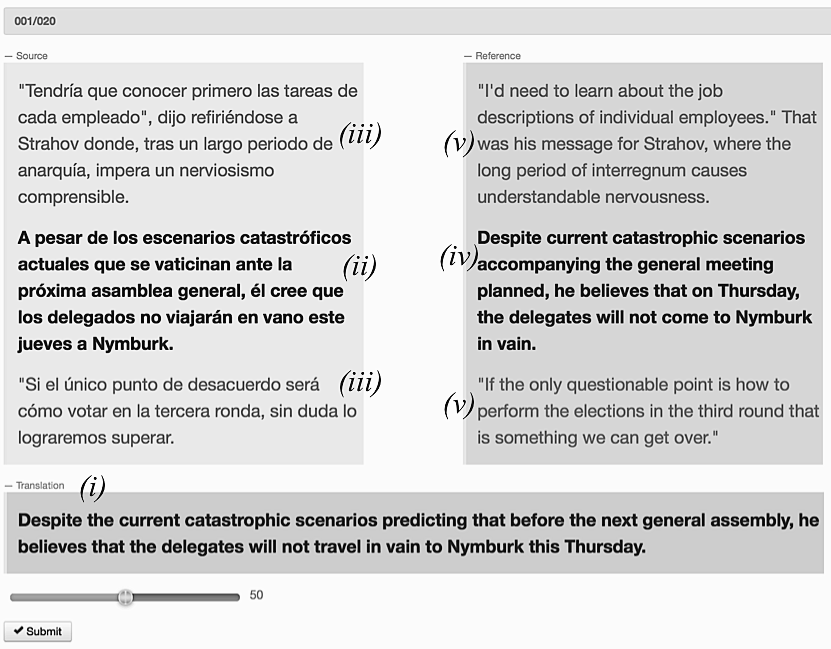
\includegraphics[scale=0.80]{data/EyeAppraiseLayout_srctgt.png}
\caption{Our modified evaluation layout showing: the translation \Ni; the source \Nii, \Niii; the reference \Niv, \Nv; and the scoring \emph{slider}.}
\label{fig:EyeAppraiseLayout}
\vspace{-5pt}
\end{figure*}

 To contrast the effect that different sources of information have on the evaluation procedure, we explored three different evaluation \gamets:
 %\vspace{5pt}

\begin{itemize}
  \item {\bf{Scenario 1}} (\src) shows participants the translated sentence (in English) along with the source text of the translation (in Spanish), including the context of the source sentence (one sentence before and one sentence after the translated sentence). 
  \item {\bf{Scenario 2}} (\srctgt) shows participants the translated sentence (in English), along with the source text of the translation (in Spanish), and a reference translation done by a human (also in English), plus context for both source and reference.  
  \item {\bf{Scenario 3}} (\tgt) shows the translated sentence (in English) only with a reference translation including its context (in English). 
\end{itemize} 
%\vspace{5pt}
%\sout{The source and the reference translation include the context of the sentence, i.e. 1 sentence before and 1 sentence after the sentence.} \stephan{redendant to scenario 1.}\\
%Explain the different layouts that were explored in our experimental design

 %was presented as a number of stars (from 0 to 5). The more stars the closer his score 
 %to the original judgment of the task sentence (See Figure ~\ref{fig:EyeAppraiseLayout}.

\subsection{Feedback}
To keep participants engaged, they were given feedback according to a previously computed quality score for each translation.  This score was calculated using a linear interpolation of the \emph{expected wins} score obtained from the ranking evaluations (normalized to the range [0, 100]) and \discoparty~\cite{discoMT:WMT2014}, a high-performing automatic MT metric based on discourse \cite{discoMT:acl2014}, which won the WMT 2014 metrics task. This was done because expected wins only provide relative scores (i.e. which of two translations is ranked better given the same source sentence), while the participants were evaluating \emph{absolute} scores.
To keep things simple, we provided feedback based on the difference between the evaluator's score and the computed quality scores. Participants were given a five scale feedback depending on the magnitude of these differences ($5$: [0--10], $4$: [11--20], $3$: [21--30], $2$: [31--40], $1$: [$>$40]). In Section~\ref{ss:disc_feedback} we analyze the impact of feedback on the evaluator behavior. %The user was given a feedback about his scoring in reference.


\subsection{Participants}

%The actual experiment was preceded by multiple rounds of pilot experiments involving 4-5 users, including the authors of this article. This step was necessary in order to fine tune the eye-tracker and exclude any external influences such as light embedding the correct recording of the eyes or noise, distracting the participants.

In our experiment we had 20 participants 27 to 45 years old. Seven of the participants were female, and 13 were male. Seventeen of our participants were computer scientists; ten had experience with manually translating documents; and four had experience with machine translation evaluation.  

%Information regarding the use of glasses/lenses (and whether they are anti-reflective) during the experiment was collected. This information was necessary to rule out any interference with the eye-tracker. due to the use of glasses or lenses. 
%Out of the 20 users, 6 wore glasses (5 were anti-reflective), and 2 users wore lenses.% Only in the case of one participant, there was interference with the eye-tracker, which could not correctly track his/her eye movements, so the participant was not taken into account.

All the recruited participants were proficient in English. However, half of the participants were recruited taking into account their mastery of the Spanish Language. For the analysis, participants were divided into two groups of ten people each: 

\begin{itemize}
  \item {\bf{Bilingual}} participants did speak the source language (Spanish) at a native or advance level of comprehension.

  \item {\bf{Monolingual}} participants did not speak the source language. Note that this group included some speakers of other Romance languages. However, the participants insisted that their understanding of Spanish was not enough to correctly comprehend the source text. 
\end{itemize}   

%The participants spoke a variety of other languages (besides the target language English), including: Arabic, Turkish, German, Danish, Bulgarian, Russian, Slovenian, Croatian, Hindi, Chinese, Basque. 
%The number of languages per person varied between 1 and 9 languages.

%A shortcoming of the experiment design was that since Spanish is a \stephan{quite expanded language ???}, our hypothesis was that the speakers of close Romance languages (such as Italian, French, or Portuguese) could partially understand the source language. For this reason, an extensive information regarding the languages participants mastered, and to what extent, was conducted. The speakers of other Romance languages, however, insisted that their knowledge of another romance language was not enough to correctly comprehend the source text in Spanish, so we ruled out this hypothesis.
%\if 0
%Out of the 10 monolingual users, 6 spoke other Romance languages, namely: 

%\begin{itemize}
%  \item 1 user spoke beginner Italian
%  \item 1 user spoke native Italian
%  \item 1 user spoke native Italian and beginner French
%  \item 2 users spoke beginner French
%  \item 1 user spoke native Portuguese
%\end{itemize} 
%\fi

\subsection{Experimental Design}
We planned our experiment to collect $1200$ evaluations, $60$ from each of the $20$ participants.  To do so, we designed an experimental matrix in which we considered the following variables: \Ni evaluator type: \mono, \bil; \Nii length of reference: \lshort, \lmid, \llong; \Niii \gamet: \src, \srctgt, \tgt; and \Niv type of translation: \qmin, \qmax.

In our experimental matrix, each participant evaluated $60$ translations evenly divided into: $20$ translations in each of the \gamet; $20$ translations from each length type; $30$ translations of each quality type. On the other hand, each translation was evaluated by four different participants, two \bil and two \mono.
To avoid any bias, we made sure that each evaluator 
%evaluated the same translation only once (or any other translation coming form the same source sentence). 
saw each source sentence only once.

%Third, we wanted to ensure that each translation is evaluated multiple times by different users.
%Explain the design matrix used. What is the total number of evaluations collected in this round? 1200, 60 per user.


\subsection{\Eye Setup}
%To conduct our experiments, we augmented Appraise ~\cite{federmann2012appraise} -an open-source toolkit ~\footnote{Available at:github.com/cfedermann/Appraise} for translation evaluation. Appraise is based on the Django web framework that uses Twitter's Bootstrap as a model for the interface design. Appraise has four different types of annotation tasks available: \Ni  Ranking (i.e. to say whether translation $A$ is better than translation $B$); \Nii Error Classification, where user classify errors in the translation output as ``minor'' or ``severe'' following \cite{vilar2006error}; \Niii Quality Estimation, where a user determines if the MT output is ``Acceptable'', ``Can easily be fixed'', or neither; and \Niv Post-Editing, where the user chooses a translation which would be the \emph{easiest} to post-edit as described in \cite{avramidis2012}.\\ 

%In our experiments 
%For our experiments, we augmented Appraise to record information from eye tracker. The new Appraise %provided in the project github repository https://github.com/guzmanhe/Appraise/
%includes the capability to interface with eye tracker and record eye information along with the user judgments. 


We used the EyeTribe eye-tracker~\footnote{http://dev.theeyetribe.com/api/} to collect \emph{gaze} information from the participants. The information was sent in messages to a modified version of Appraise\footnote{Available at: https://github.com/Qatar-Computing-Research-Institute/iAppraise} at a rate of 60Hz (a packet in every 16ms). 
%information and communicate the data to the \eye server which serve to broadcast the data/messages read by device to Appraise.  %Communicating with the tracker server is achieved using a connection via a TCP socket that listen to the designated server port (Eyetribe default port 6555). The Tracker API protocol consists of exchanging JSON (JavaScript Object Notation) formatted messages over TCP sockets\ahmed{Figure sample packet}. 
%

Each message contained the gaze position in the screen of both eyes, a flag indicating if the point represented a \emph{fixation}, a time stamp, and other device-related information. 
%a state indicating the status of the tracker. EyeTribe user guide~\footnote{http://dev.theeyetribe.com/api/} details further the structure and the attributes of the messages that can be exchanged with the server. %Figure \ref{fig:EyetribeAPImap}. details the architecture of Appraise. The Eyetribe device was set to operate at a frequency of 60Hz (a reading in every 16ms) which makes it not suitable to track \stephan{high accuracy? Is this the accurate term?} saccades. 
%The screen was configured in a \paco{Ahmed can you add resolution here}, resolution.
%
To ensure optimal readings, participants were asked to calibrate the \eye device before starting the experiments, and a warning message was displayed whenever the eye-tracker lost track of the participant's gaze.
%\begin{figure}[ht]
%\centering
%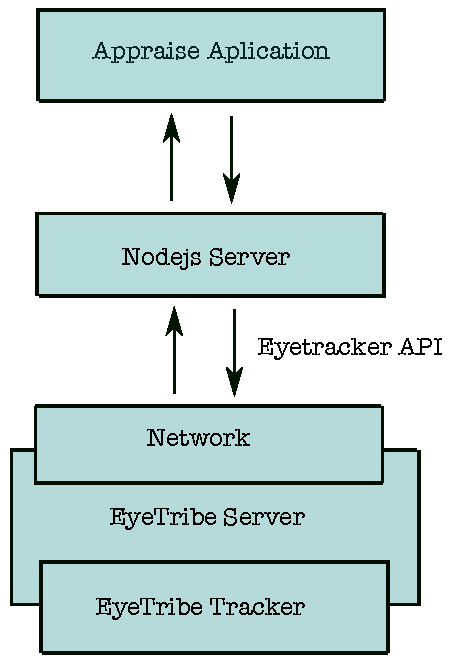
\includegraphics[scale=0.6]{data/EyetrackingAPI.pdf}
%\caption{Eyetribe communication map}
%\label{fig:EyetribeAPImap}
%\end{figure}


%What was the device used for \eye? Can we give more specs (paragraphs only). \paco{@Ahmed}


\subsection{Instructions and Exit Survey}


%
%tuning the eye-tracker required sitting at a certain distance from the computer screen, and looking with both eyes towards the eye-tracking software until the software would recognise both eyes of the participant. 
%Next, the participant had to follow with his/her eyes a moving red circle, in order to train the software to recognise the movement of his eyes. As a third step, the eye-tracking software would show its performance by colouring in red the spots on the screen on which the participant would look at. The objective was to reach 5 stars of calibration, and the software would allow re-calibration if the sufficient quality was not reached (see Figure ?). 

%The latter %The tutorial introducing the experiment 
%would present to the participant the three scenarios and instructions on how to navigate through the screen. %(see Figure? ). 
%
%
Participants were asked to move as little as possible to not interrupt the readings of the eye-tracker, 
%
%
%explicitly asked to not move away from the screen while performing the experiment, as the eye-tracker could lose their eyes. 
%They were also asked 
%
%
and to not interrupt their work while working through the translations belonging to one \gamet, as the time for executing all sentences in one scenario was measured. 
Before conducting the evaluation, participants were shown two tutorials, one showing how to calibrate the eye-tracker and one showing how to conduct the experiment. 

After the tutorials they were asked to perform a warm-up exercise consisting of %2 
two sentences per \gamet.  
%\ahmed{Chop-off all the intro, too much details, no space.}
Then, the participants proceeded to evaluate the $20$ translations in each of the \gamets in the following order \src, \srctgt and \tgt \footnote{In hindsight, randomizing the order in which the \gamets were performed would have allowed to answer an additional set of questions.}.

%What were the considered variables?
%\paco{@Irina}
%\subsubsection{Exit survey}
After the experiment, the participants were asked to fill in an on-line exit survey, which collected their impressions about the experiment and their physiological status during the experiment.

%\begin{itemize}
%  \item Their cognitive state during the experiment (normal, tired, sleepy, sleep-deprived, sick/dizzy);
%  \item The interface;
%  \item The difficulty of evaluating the translation;
%  \item The environment;
%  \item Other.
%\end{itemize}

%A screenshot of the survey form is shown in Figure?. 
From the survey we learned about the physiological state of the participants: $55\%$ of them were in a normal state, $15\%$ were slightly tired or sleepy, $25\%$ were tired, and $10\%$ were sleep-deprived or sick. Yet, all these reports were evenly distributed among \bils and  \monos.
%11 participants were in ``normal'' state, 2 were ``normal, sleepy'', 1 was ``normal, tired'', 5 were ``tired'', out of which 2 were ``tired, sleepy''. 1 was ``sleep-deprived'' and 1 was ``sick/dizzy''. 
%Regarding the interface, participants were mostly content with the experiment {\bf{interface}}, defining it ``clear'', ``simple'', ``easy to use'', and ``very intuitive''. 
%However, $15\%$ of the participants complained of being distracted by a warning message that appeared when they moved away from the eye-tracker,
%the fact some texts where very long %so they had to scroll up and down, 
%or the fact that they had to stay focused on the same screen for too long without moving their eyes.% 3-4 participants also complained of the fact that there were people discussing around them (the experiment was done in an university environment). 

%The perceived \emph{difficulty} of the evaluation task ranged widely among participants (from very easy to hard).

 There were only few complaints about the setup, and they were related to: \Ni the lack of precise instructions of what constitutes a \emph{good} translation, \Nii the large range of the evaluation score (0-100), \Niii the difficulty to understand the context of the translations, and \Niv the cognitive overhead needed to evaluate \llong translations, especially in the \srctgt \gamet. As expected, some of the \mono participants noted that in the \src \gamet they mostly evaluated the readability of the translation, as they had no knowledge of the source language.
\vspace{5pt}



\section{Results}
%!TEX root = main.tex

%\paco{Ahmed is going to work on a pre-version of this by adding all the graphs}
In this section we analyze the process that participants use to evaluate translation. We focus on three different aspects. First, we use \eye data to observe in which areas do participants spend most of their time. Next, we analyze the time that participants take to complete the evaluation. Finally, we analyze the scores given by the participants, and their consistency.

\vspace{5pt}
\subsection{How Long Does it Take?}
\vspace{5pt}

One important aspect to take into account is the time at which annotations can be collected \cite{callisonburch-EtAl:2007:WMT}. To discount the time a participant spends idle (be either by fatigue, distraction, etc.), here we analyze only the \emph{focused} time, i.e. the amount of time a participant gaze is focused in \emph{areas of interest}.
\\
 In our experiments, we observed that on average annotations take $26.06$  seconds to be collected, which is in line with the measurements reported by \newcite{callisonburch-EtAl:2007:WMT}. In Table~\ref{tab:time-length}, we further break down the task durations by: \Ni type of evaluator (i.e. \mono and \bil), \Nii \gamet (i.e. \src, \srctgt, and \tgt); and  \Niii the length of the source sentence (i.e. \lshort, \lmid, \llong).


\begin{table}[htb]
\vspace{5pt}

\small
\begin{tabular}{rllrrrr}
  \toprule
 & scnr. & usr\_type & \llong & \textit{med} & \lshort & avg \\ 
  \midrule
1 & src & biling & 36.89 & 24.54 & 17.92 & 26.46 \\ 
  2 & src & mono & 44.11 & 28.58 & 19.17 & 30.55 \\ 
  3 & src+tgt & biling & 40.16 & 23.99 & 15.46 & 26.59 \\ 
  4 & src+tgt & mono & 46.76 & 29.69 & 21.63 & 32.71 \\ 
  5 & tgt & biling & 26.41 & 15.03 & 10.54 & {\bf 17.28} \\ 
  6 & tgt & mono & 35.90 & 19.41 & 12.69 & 22.77 \\ 
   \bottomrule
\end{tabular}
\caption{\label{tab:time-length}Average task duration time (in seconds) according to type of setup, type of evaluator and source sentence length.}
\vspace{5pt}

\end{table}


The first observation to make is that \bil evaluators are consistently faster than \mono evaluators in evaluation. This is true even in the \tgt condition, where both evaluators can leverage the same amount of information (i.e. both are fluent in English). %\paco{ I DONT KNOW IF THIS SHOULD GO HERE OR LATER.} 
This can have two possible explanations: \Ni \bil evaluators develop \emph{internal} rules that allow them to perform the task faster, and \Nii since the order of the conditions was fixed (i.e evaluators performed first the \src tasks, then the \srctgt tasks and lastly the \tgt tasks), this could mean that the \bil evaluators got \emph{more efficient} sooner, just because the \src task wasn't noise to them. However, we show later that \Ni is more plausible.

The second observation to make is that evaluators tend to take longer to evaluate scenarios with more sources of information available. This is true for \mono if we analyze the results either by \gamet or by source length\footnote{Longer source sentences have more words.}. Surprisingly, \mono participants in the \src condition perform the task $7\%$ faster than in the \srctgt condition, which leads to hypothesize that the more information is in the screen, the longer the task will take, even if the information is not particularly useful for the task completion. On the other hand \bil take the least time when evaluating \tgt scenario.\\ %\irina{This observation has been confirmed by the final feedback provided by the participants (see Section 2.6)}.

To measure the significance of our observations, we fitted a random intercepts model  and analyzed the relationship between task duration time, length of the sentences, type of evaluator and type of scenario while taking into account the variability between evaluators. Therefore, as fixed effects, we had the length of the sentences, the type of evaluator (\bil and \mono) and the \gamet into the model. We also included the interaction between the type of evaluator and the length of the sentences. As random effects, we had intercepts for each of the 20 evaluators. P-values were obtained by likelihood ratio tests of the full model with the effect in question against the model without the effect in question. 
\vspace{5pt}

In general, the effect of \gamet is highly significant ($\chi^2_{2}=121.71$, $p=2.2e^{-16}$), and for long sentences the \tgt scenario is $8.52$ and $9.6$ seconds faster than the \src and \srctgt scenarios, respectively. The effect of the type of evaluator is also significant  ($\chi^2_{3}=7.45$, $p=0.05$), and on average \bil are faster than \mono by $7.76$ seconds for long sentences. These results were obtained using R \cite{R:2015} and lme4 \cite{LM4:2015}, following \newcite{DBLP:journals/corr/Winter13}.


%Analyzing evaluator's speed from Figures ~\ref{fig:TimeScoremax} and ~\ref{fig:TimeScoremin}, shows that bilingual evaluators are relatively faster in completing tasks for both max and min types. Bilingual mean, max is (27.51,64.91) versus (33.78,121.65) for the Monolinguals. Monolingual evaluator's speed varies widely. Scoring ``max'' category takes more time for both evaluator types.
%Here we evaluate how evaluators's speed is, and how does it affect results if any.
%\begin{figure}[ht]
%\centering
%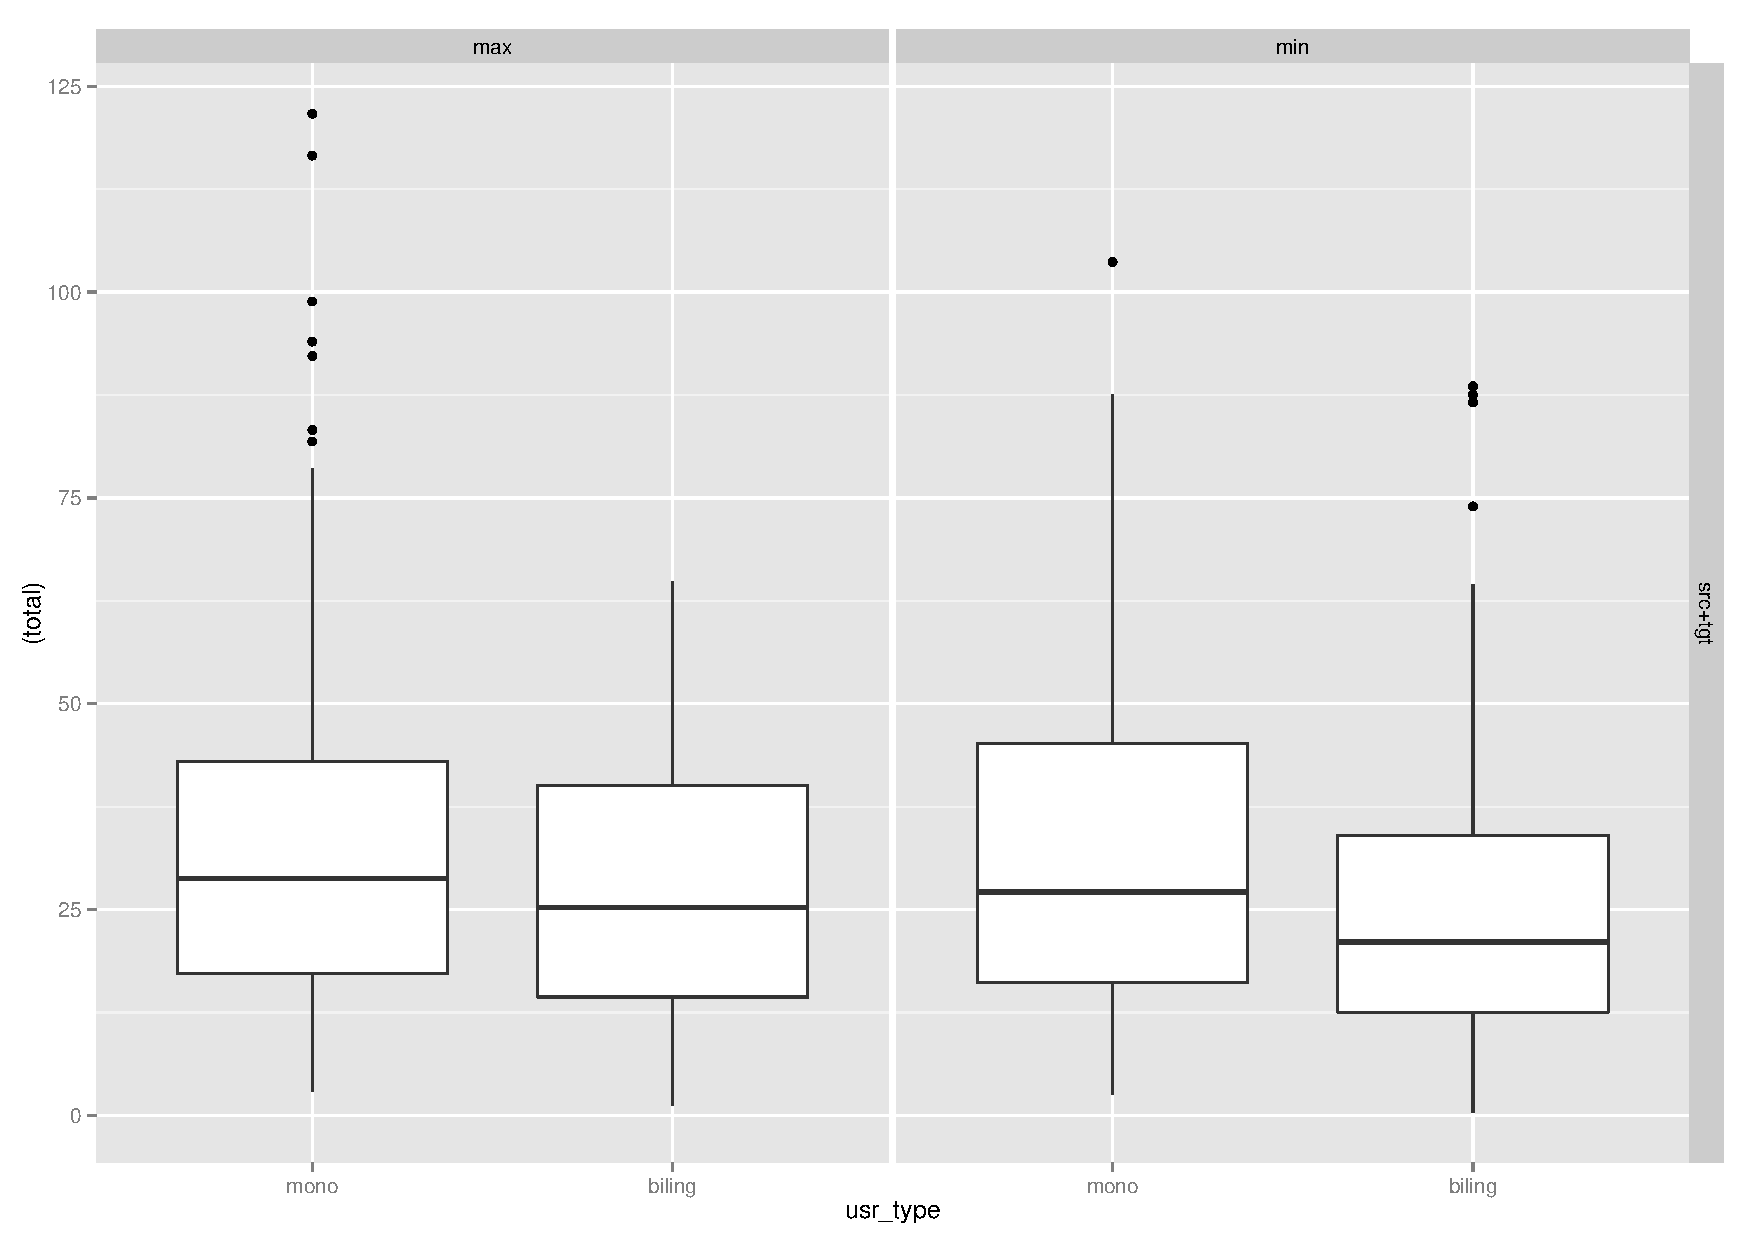
\includegraphics[scale=0.265]{data/time_srctgt.pdf}
%\caption{Users time in src+tgt scenario}
%\label{fig:TimeScoremax}
%\end{figure}


\vspace{10pt}
\subsection{Where Do Evaluators Look?}
\vspace{5pt}

The \eye data allowed us to analyze the behavior of the evaluators across different conditions. In particular, we focused in the \emph{dwell} time, i.e. the amount of time an evaluator is looking at a particular \emph{area of interest} in the screen. In Table~\ref{tab:aoi}, we present the proportional \emph{dwell} time (out of the \emph{focused} time) that the evaluators spent in the different areas of the screen: \Ni translation, \Nii source (with previous and next context), \Niii reference (with previous and next context), \Niv and the sum of the source and reference times.\\



\begin{table}[ht]
\centering
\small
\begin{tabular}{rllrrrr}
  \toprule
 & scnr. & usr\_type & tra & ref & src & src+ref \\ 
  \midrule
1 & src & mono & 0.18 & - & 0.82 & 0.82 \\ 
  2 & src & biling & 0.12 & - & 0.88 & 0.88 \\ 
  3 & src+tgt & mono & 0.13 & 0.24 & 0.63 & 0.87 \\ 
  4 & src+tgt & biling & 0.07 & 0.16 & 0.78 & 0.93 \\ 
  5 & tgt & mono & 0.26 & 0.74 & - & 0.74 \\ 
  6 & tgt & biling & 0.19 & 0.81 & - & 0.81 \\ 
   \bottomrule
\end{tabular}
\caption{\label{tab:aoi} Proportional time spent by evaluators while focusing in different regions of the screen: translation (trans), reference and its context (ref), source and its context (src), and the aggregate of src and ref.}
\end{table}

%\\
From the table, the main observation is that evaluators spend most of their time looking at regions other than the translation (src+ref). This supports the hypothesis that evaluators try to understand the source and reference before making a judgment about the translation. However, there are some peculiarities worth noting. First, \bil participants spend less time reading the translation than their \mono counterparts. %This is particularly noticeable in the \srctgt condition, where \bil evaluators spend about $78\%$ of their time reading the source(s), and only $7\%$ of their time reading the translation. 
\\
\pagebreak
\vspace{10pt}

For example, this means that on average, in the \tgt condition, a \bil evaluator would spend  $5$ ($0.19*26.41$) seconds\footnote{This time does not need to be continuously spent on the same region. For example, a evaluator might analyze a first portion of a translation, then move back to the reference, and then return to the translation.} focused on a \llong translation while a \mono evaluator would spend $9.3$ ($0.26*35.9$) seconds, that is almost \underline{double} the time. In contrast, the difference times both \bil and \mono evaluators would spend reading the reference is only a factor of $1.2$ ($21.3$ and $26.6$ seconds, respectively). This tells that \bil are faster (mostly) because they spend \emph{less} time reading the translation.

Another interesting observation is that \mono spend a sizable proportion of their time reading the source (which they supposedly \emph{do not} understand), even in the \srctgt scenario. This suggests that \mono evaluators develop \emph{rules-of-thumb} to analyze the source, even if it is a foreign language (e.g. translation of named entities, numbers, dates). This can be an artifact of the relatedness between English and Spanish, or an priming effect induced by the order in which the tasks were done (i.e by asking \mono evaluators to score \src tasks first, we forced them into developing this behavior). The analysis of such phenomena, while interesting, is beyond the scope of this paper.

Finally, if we look across conditions, we observe that evaluators spend a larger proportion of their time evaluating the translation in the \tgt condition than in the \src and \srctgt conditions. Yet, when we calculate the expected focused time in the translation region for each condition (across different lengths and evaluator types), we obtain $4.48$, $4.35$ and $2.85$ seconds for each condition, respectively. \\


This tells us that having more information on the screen (the case of \srctgt) decreases the total amount of time spent reading the translation. In other words, if a evaluator has more sources of information to evaluate a translation, s/he'll spend more time performing the task, but less time evaluating the translation itself. 

% The data collected showed that background of evaluators has an impact on translation. While both evaluators type (mono- and bi-linguals) uses all the information available to them as shown in Figure ~\ref{fig:evaluatorsregionsmin} and ~\ref{fig:evaluatorsregionsmax}; both they tend to use the information is different way depending on the game and quality. In the next sections, we will dive deeper on the various aspects of these differences trying to answer our research questions and reveal key information about the evaluation process. 
% \begin{figure}[ht]
% \centering
% 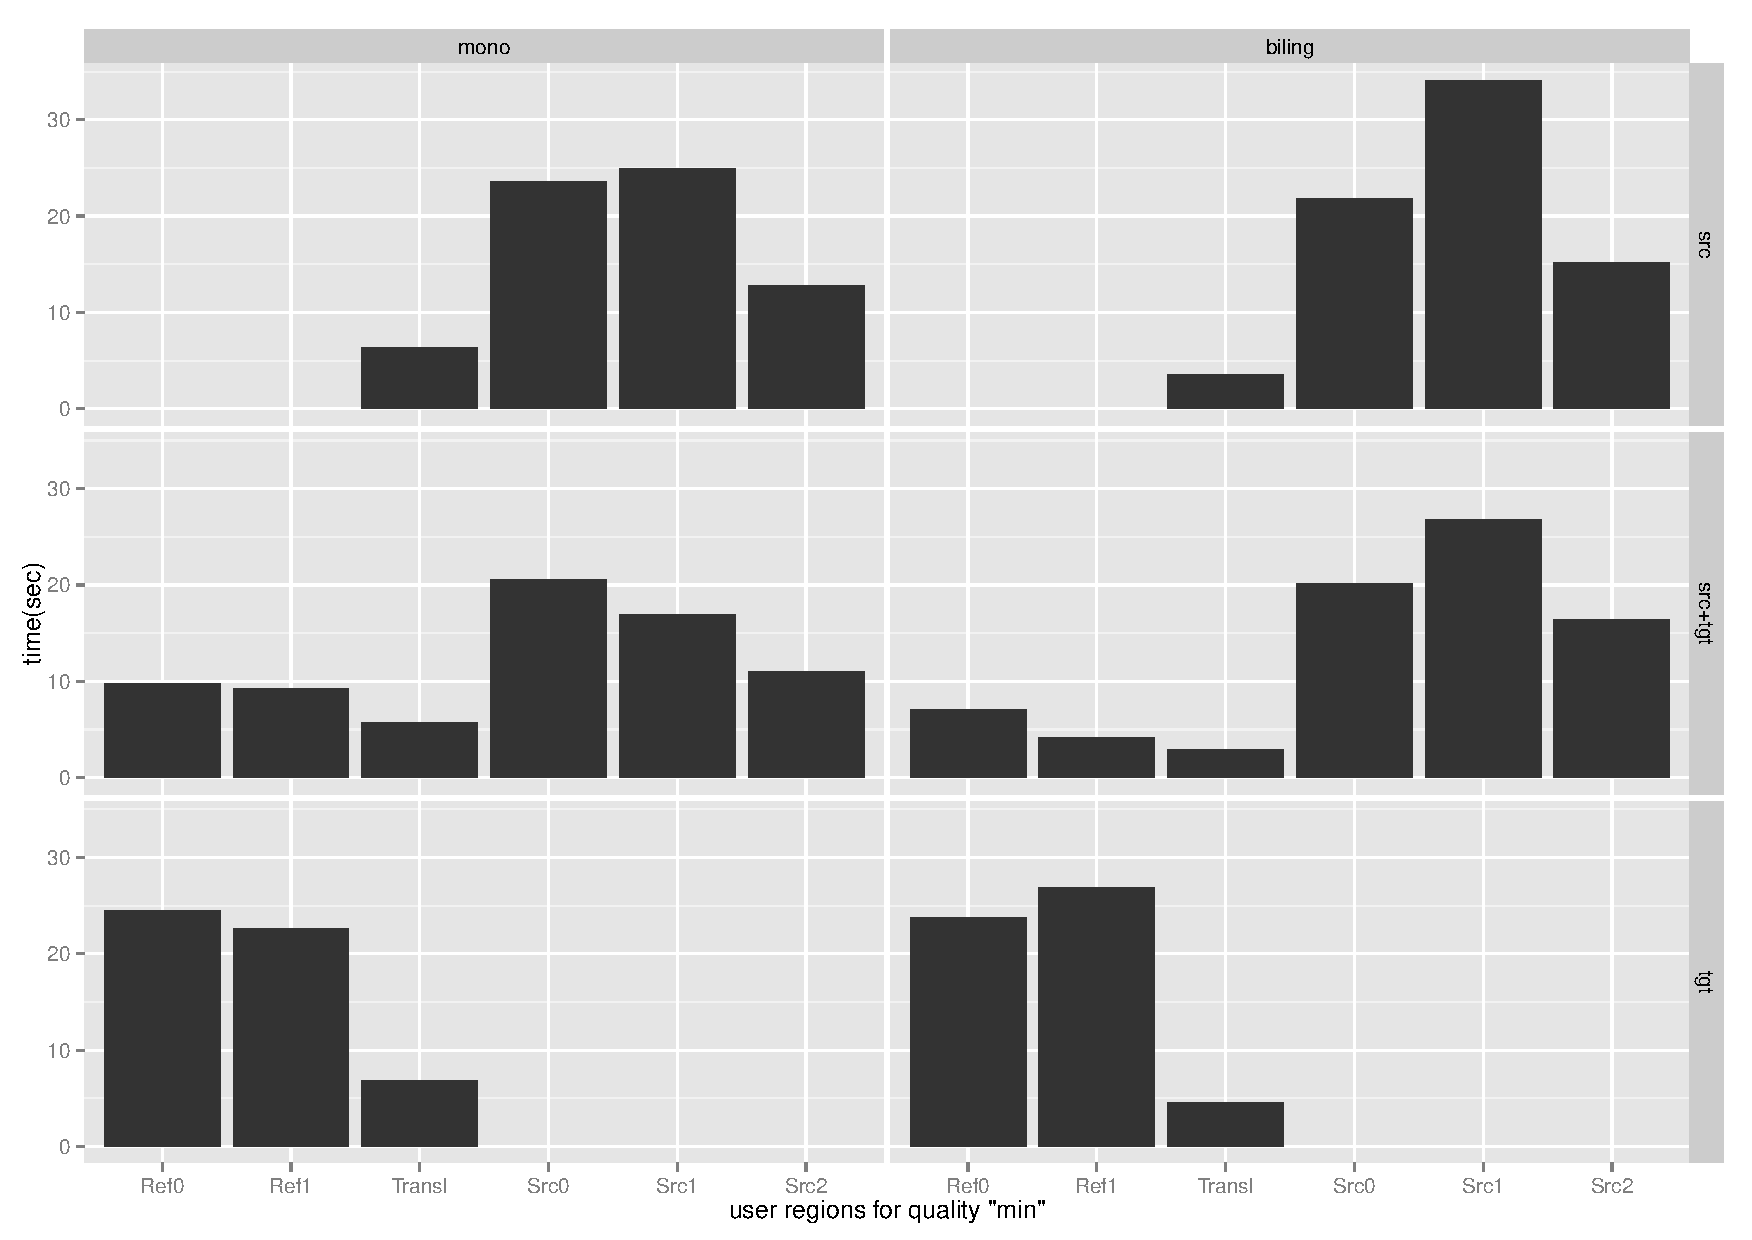
\includegraphics[scale=0.275]{data/Users_regions_min.pdf}
% \caption{Users time in regions while scoring ``min'' category.}
% \label{fig:evaluatorsregionsmin}
% \end{figure}
% \begin{figure}[ht]
% \centering
% 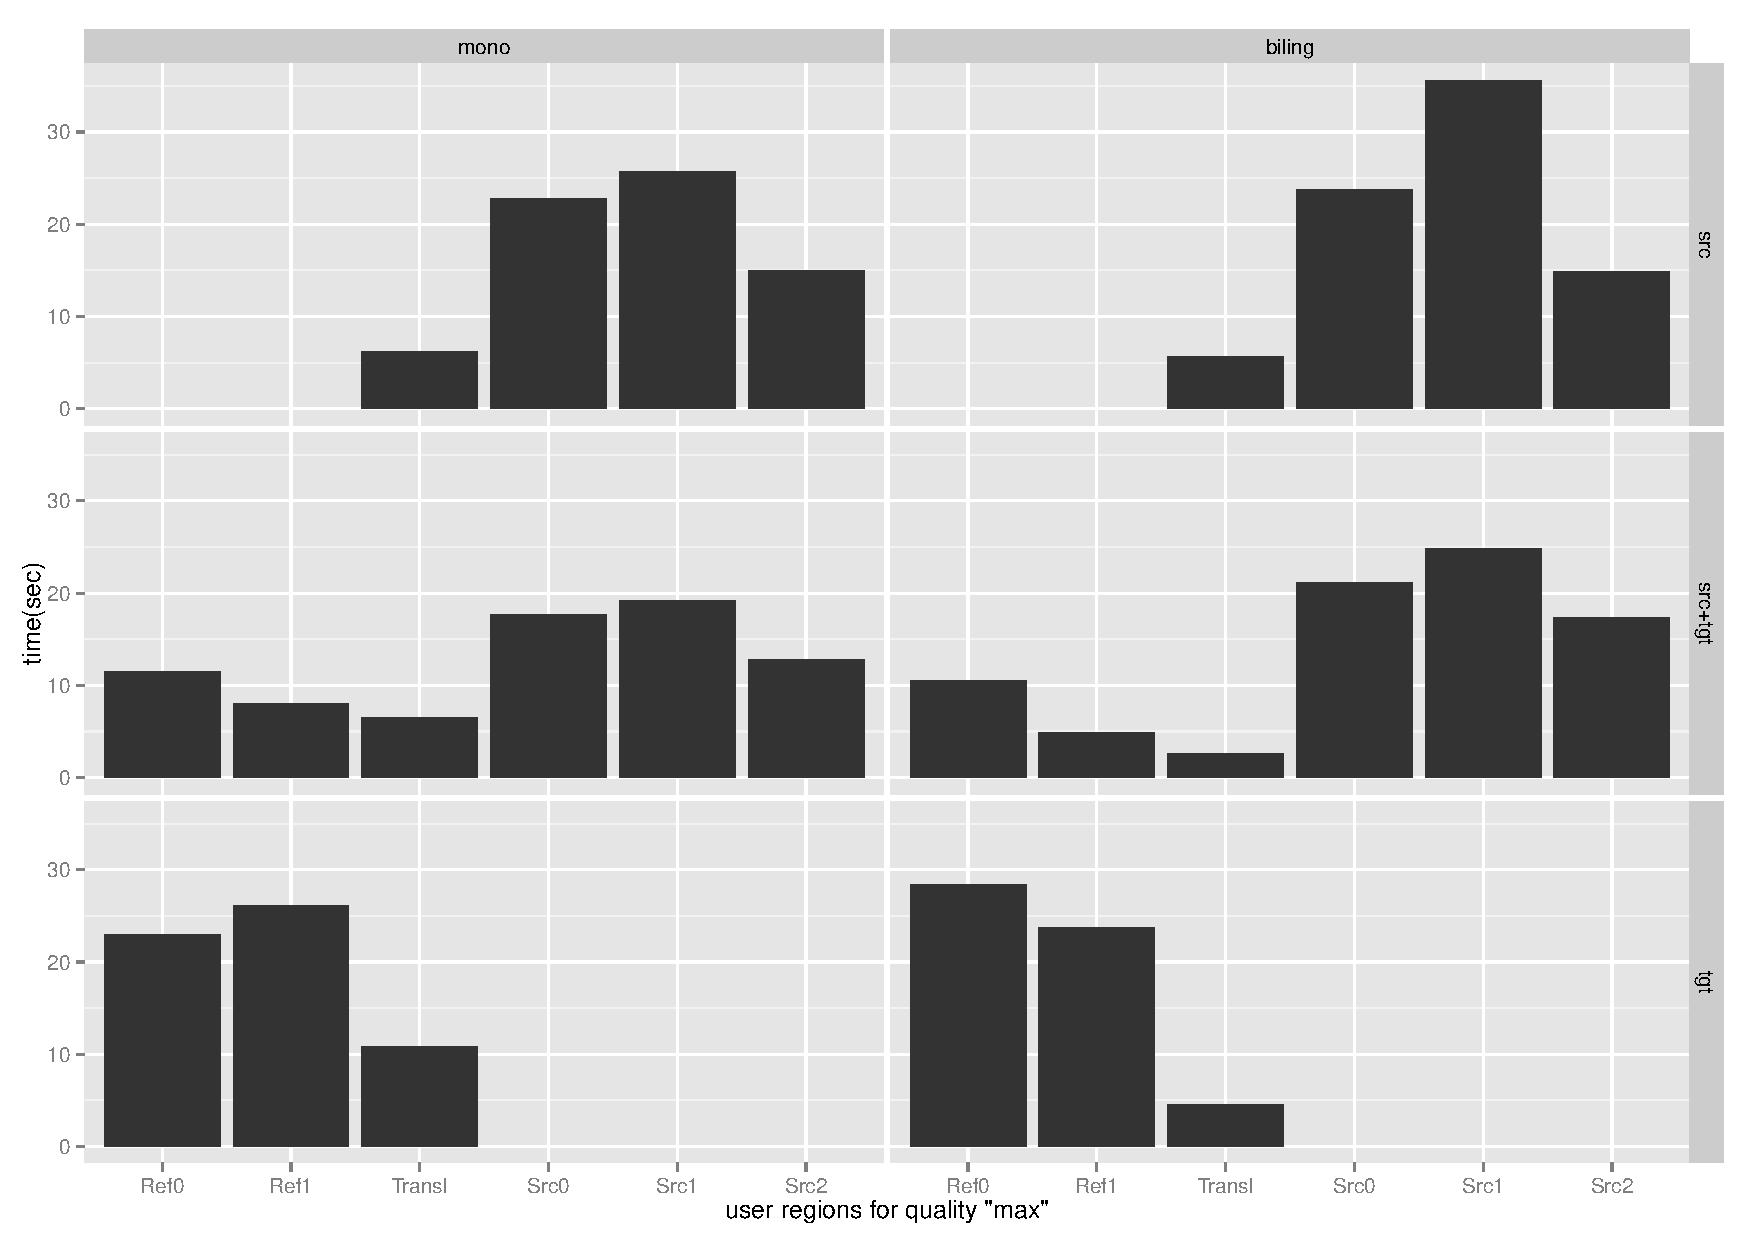
\includegraphics[scale=0.275]{data/Users_regions_max.pdf}
% \caption{Users time in regions while scoring ``max'' category.}
% \label{fig:evaluatorsregionsmax}
% \end{figure}

\vspace{3pt}
\subsection{Score Consistency} 
Another important aspect to take into account is how consistent are the scores provided by different evaluators, and how this consistency varies depending on the type of evaluator, and the \gamet that is used. Unlike other studies where categorical and ordinal scores are produced, here each annotation generates a score in a continuous scale\footnote{Actually it is an ordinal scale from 0-100, but for practical purposes we treat it as continuous}. Thus, using the standard inter-annotator agreement is impractical. Instead, we evaluate \emph{consistency} as the standard deviation of scores for each translation with respect to a class or group average (i.e. \mono or \bil). This quantity gives us an idea of how much variation there is in the score for a specific translation across different groups of evaluators. To be able to compare across evaluators, we  normalized their individual scores to a 0-1 range using \emph{minmax}. Then, computed the consistency as follows:

\begin{equation}\label{eq:1}
\sigma_c^2 =   \frac{1}{N_c}\sum_{i \in T} \sum_{j\in C} (\tilde x_{ij} - \bar{\tilde x}_{ic})^2
\end{equation}

\noindent where $\tilde x_{ij}$ is the \emph{normalized} score of translation $i$ by an evaluator $j$ who belongs to class $c$ (e.g. \mono), and $\bar{\tilde x}_{ic}$ is the average score given to translation $i$ by evaluators in class $c$, and $N_c$ is the total number of translations scored by evaluators in class $c$. \\

In Table~\ref{tab:consistency} we present the consistency measurements for \mono and \bil evaluators across the different conditions. 

 %We measured the consistency between evaluators \emph{cost}, group \emph{cost\_group} and versus original scores \emph{hum\_cost} as shown in Figure~\ref{fig:evaluatorconsistency}. Monolinguals shows that they are more consistent (\emph{lower cost}) cross all \gamet{s}. 


\begin{table}[ht]
\centering
\small
\begin{tabular}{rllr}%}
  \toprule
 & scnr. & usr\_type & $\sigma_c$  \\%& $\tau_c$ \\ 
  \midrule
1 & src & mono & 15.14 \\%& 28.79 \\ 
  2 & src & biling & 16.17 \\%& 29.74 \\ 
  3 & src+tgt & mono & 14.88 \\%& 27.04 \\ 
  4 & src+tgt & biling & 15.96 \\%& 26.22 \\ 
  5 & tgt & mono & {\bf 14.13} \\%& {\bf 24.73} \\ 
  6 & tgt & biling & 16.81 \\%& 27.62 \\ 
   \bottomrule
\end{tabular}
\caption{\label{tab:consistency}Consistency scores: standard deviation with respect to the class average ($\sigma_c$) %and with respect to the human ranking scores ($\tau_c$) 
for the scores produced by different types of evaluators across different conditions. Lower scores means higher consistency. Each measure is calculated over $N=200$ points.}
\vspace{-10pt}
\end{table}

First note that \mono evaluators are more consistent within their group ($\sigma_c$) than the \bil evaluators. This observation holds true across all the different scenarios. Note also that \mono evaluators are the \emph{most} consistent in the \tgt condition.  We hypothesize that this is due to the longer times spent analyzing the translation in comparison to \bil evaluators. But also, we think this is related to the simplicity of the task. There is less information to analyze. On the other hand \bil, have a larger variation, which can be attributed to the heterogeneity of \emph{rules of thumb} that the evaluators develop from looking at the source.
%Also note that \mono users in the \tgt have the least deviation from the \emph{corrected} human ranking scores, which tells us that the user scores are more in agreement with the rankings provided in the WMT12 tasks for the same translations.
Finally, note how \bil have a problem of consistency with the \tgt task. Without more fine-grained information, we can only hypothesize that this is due to the lack of familiarity with the scenario. Before performing tasks in the \tgt scenario, they were relying primarily on the source to evaluate.% This can be due to the %Here we tell how users are consistent with each other and with the ranking/provided scores

%\begin{figure}[ht]
%\centering
%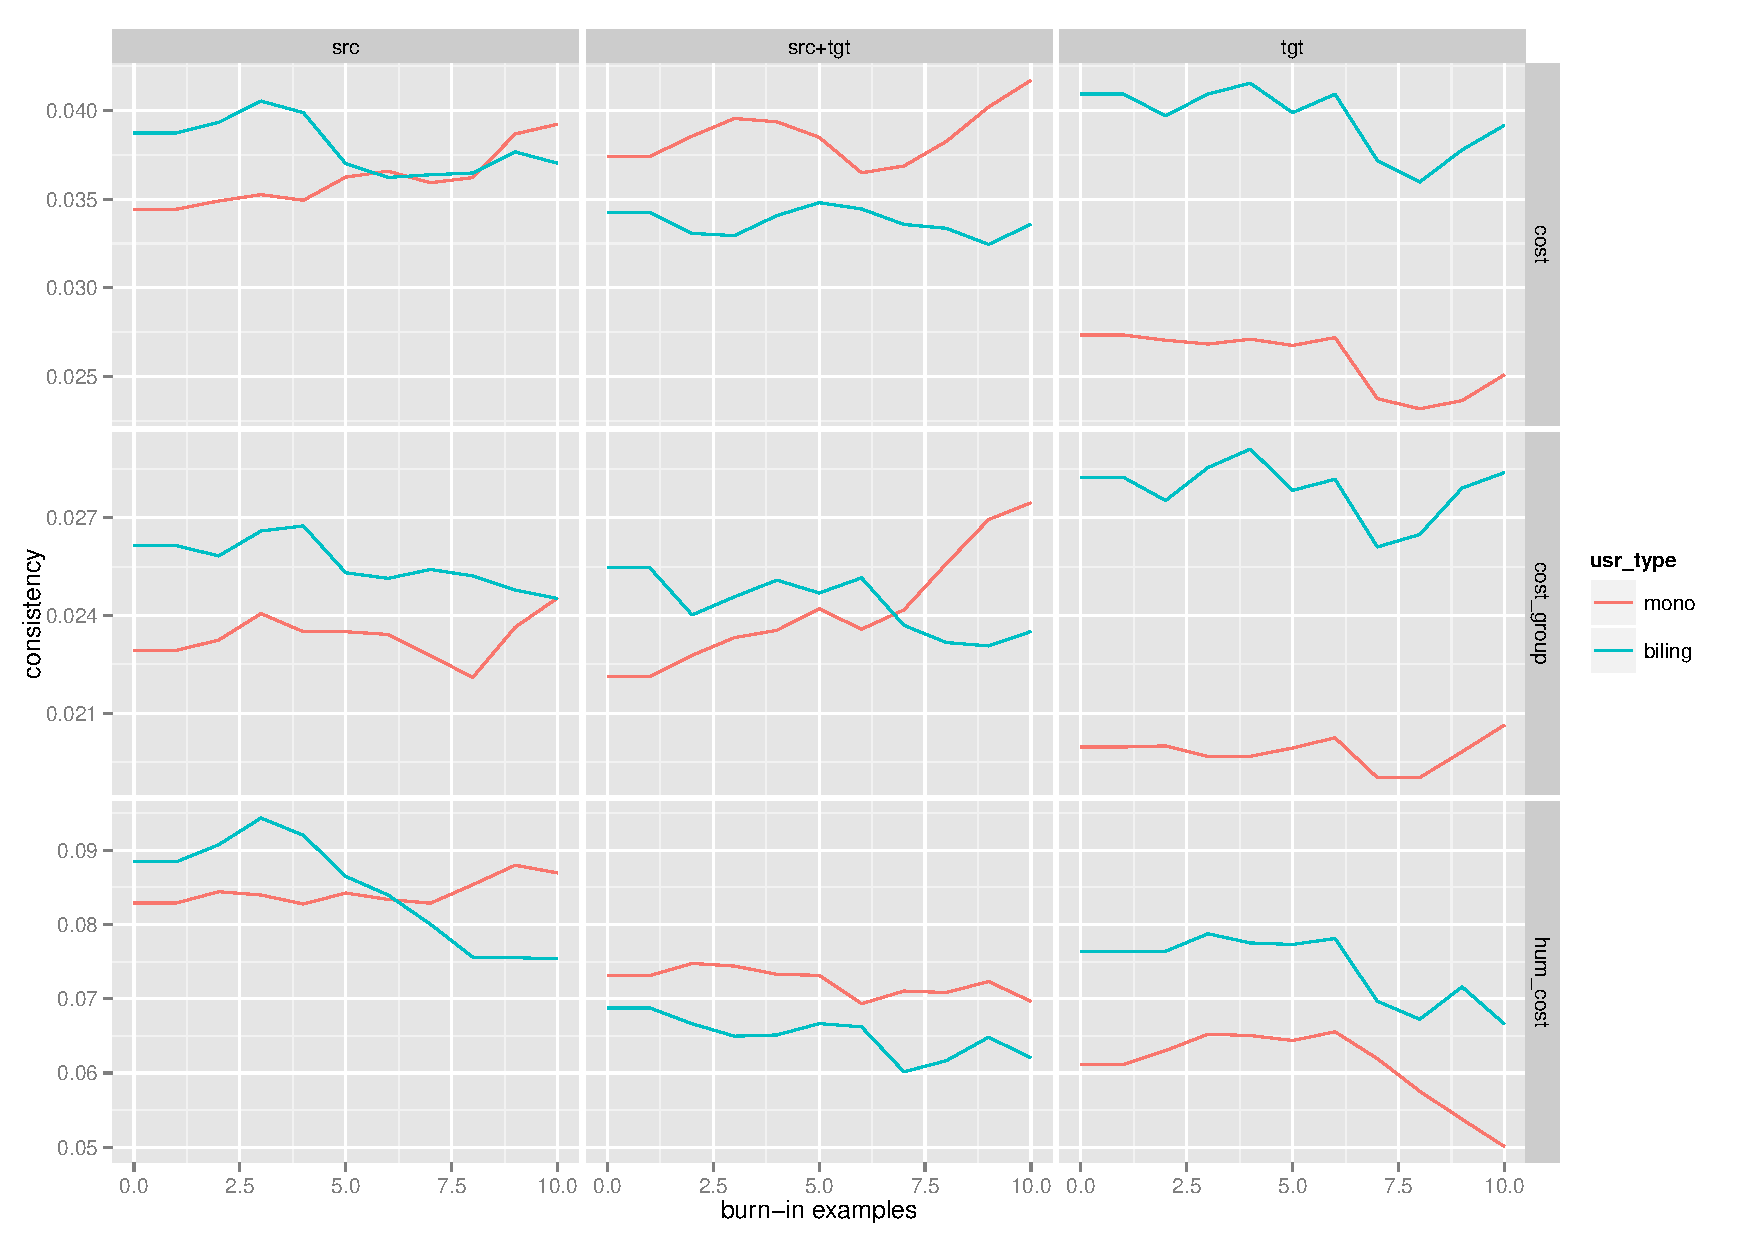
\includegraphics[scale=0.29]{data/consistency.pdf}
%\caption{Users consistency in various scenarios}
%\label{fig:userconsistency}
%\end{figure}

\subsection{Summary of Observations}
We have observed that there are differences in how translations are evaluated according to the type of evaluator, and the scenario. In summary, the observations are:
\begin{itemize}
\item The \bil evaluators perform the tasks faster than the \mono. They also spend less time evaluating the translation.
\item The \mono evaluators are slower, but more consistent in the scores they provide. %When only the source information is displayed, \mono evaluators still 
\item The more information is displayed in the screen, it will take to longer to complete the evaluation, even though, less time will be spent actually evaluating the translation. Displaying more information also correlates with lower consistency between evaluators.
\end{itemize}

% \subsection{User Behavior}
% %Here we discuss how users evaluate. 
% Figures ~\ref{fig:behavbilgmax} and  ~\ref{fig:behavmonomax} present the users behavior while evaluating sentences from ``max'' category. The circles size represents the proportional time spent in the area while the directed arcs width reflect the frequency of the transition between the connected regions. From the figures, we can note that the bilingual users tend to spend more time between source -See Figure ~\ref{fig:behavbilgmax}- regions when compared to monolinguals. Monolinguals move back and forth between source and reference more frequently when scoring ``max'' category as shows Figure ~\ref{fig:behavmonomax}.
% %What are the differences across regions in the layout
% \begin{figure}[ht]
% \centering
% 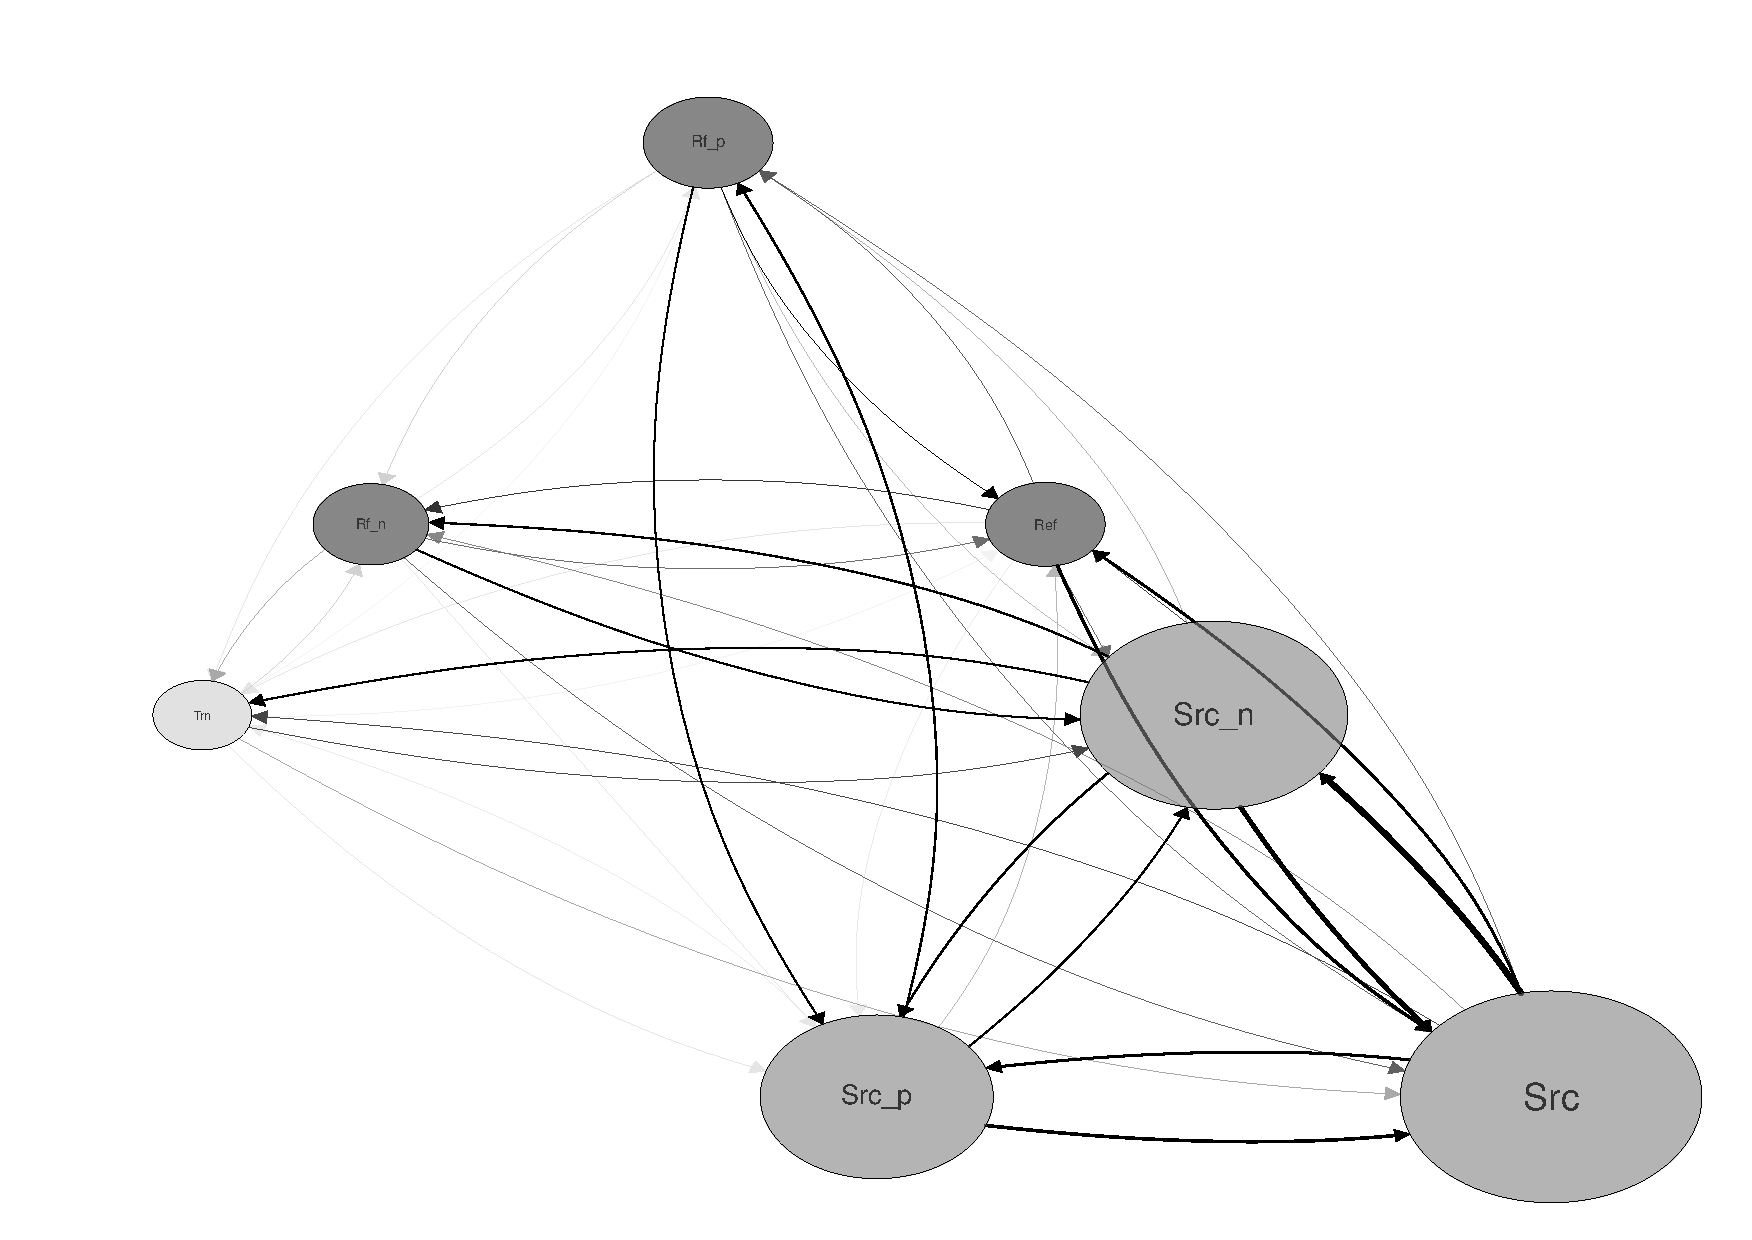
\includegraphics[scale=0.27]{data/behav_bilg_srctgt_max.pdf}
% \caption{Bilingual user process of scoring ``max'' category.}
% \label{fig:behavbilgmax}
% \end{figure}
% \begin{figure}[ht]
% \centering
% 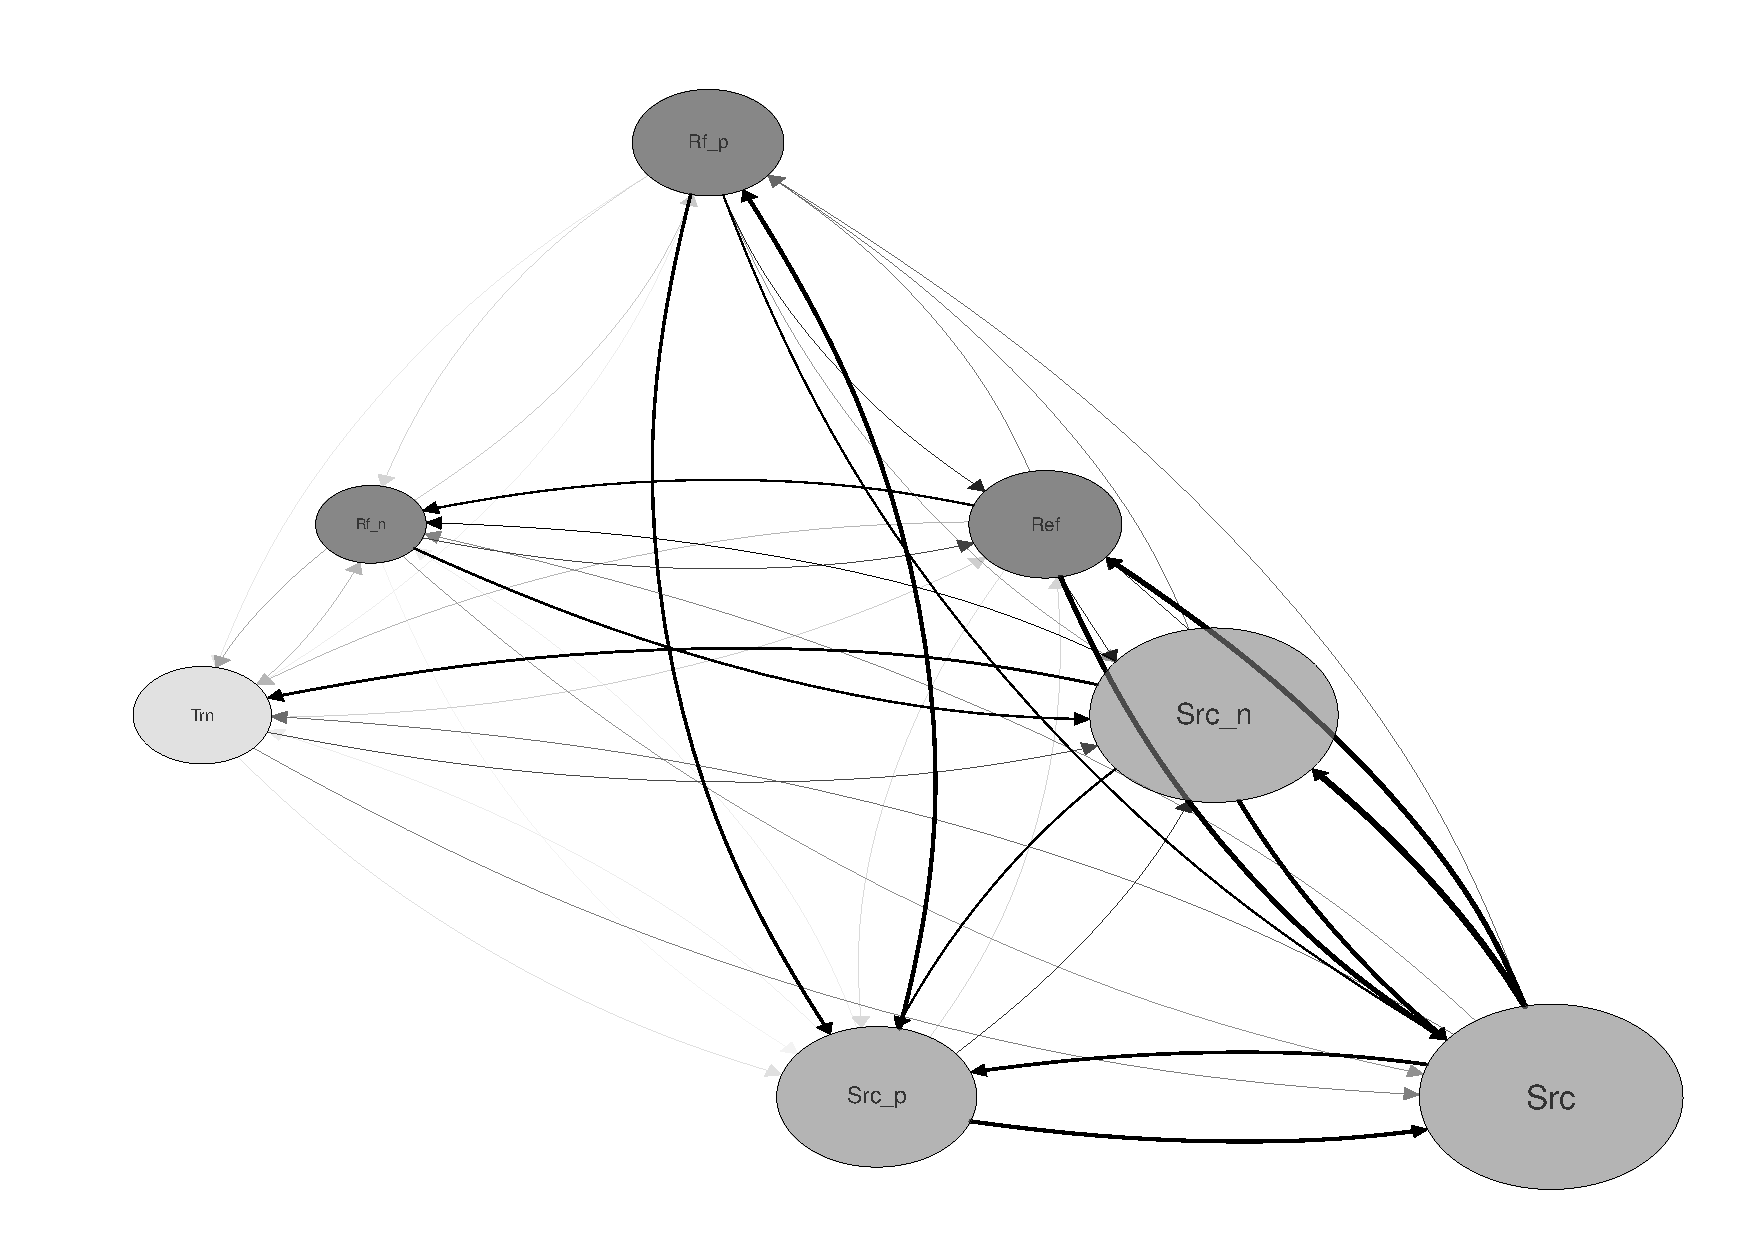
\includegraphics[scale=0.27]{data/behav_mono_srctgt_max.pdf}
% \caption{Monolingual user process of scoring ``max'' category.}
% \label{fig:behavmonomax}
% \end{figure}
% \\
%\if 0
% Conclusions:\\
% The results shows that while bilingual evaluators are typically faster that their monolingual peers, the latters are more consistent in their judgments. Monolingual inability to access source data, it is not an obstacle for them to make an accurate judgment.  On the other hand, when the hypotheses were scored with a language model. Monolingual looks like they are more consistent in mimicking language model scores as shown in Figure ~\ref{fig:costlm} -Dashed lines. 
% \begin{figure}[ht]
% \centering
% 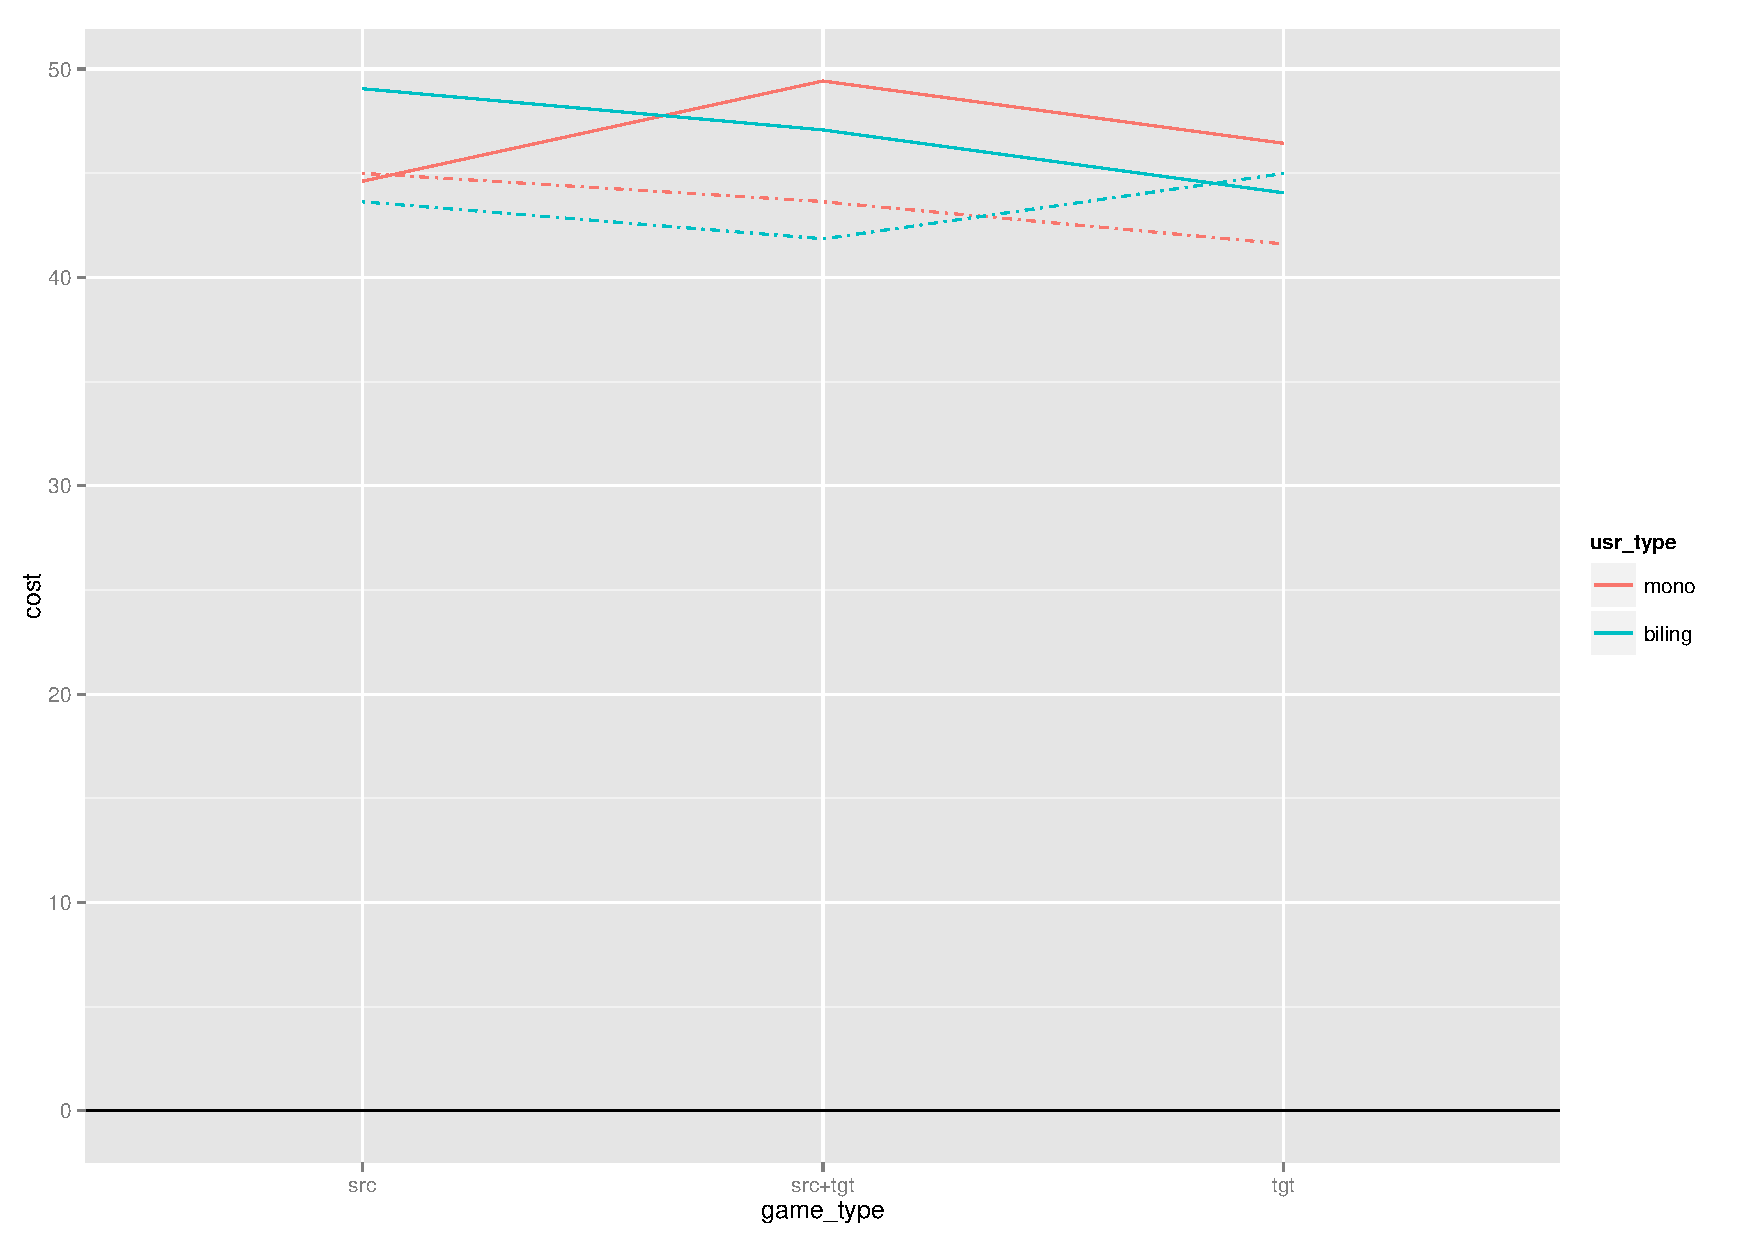
\includegraphics[scale=0.26]{data/cost_users_lm.pdf}
% \caption{Consistency of users vs humans and language model}
% \label{fig:costlm}
% \end{figure}
% %\fi

%So far, no huge difference between HIGH/LOW


\pagebreak
\section{Discussion}
%!TEX root = main.tex
 Using \eye allowed us to dive into the process of evaluation and explore new aspects regarding the behavior of evaluators. However, there were a few additional questions that might arise from our setup and experimental results. In this section we address some of them. %The experiments we conducted allowed to report the following findings related to our research questions. 
% \if 0
% The results shows that while bilingual evaluators are typically faster that their monolingual peers, the latters are more consistent in their judgments. Monolingual inability to access source information, did not appear to be an obstacle for them to make an accurate judgment.  On the other hand, when the hypotheses were scored with a language model. Monolingual looks like they are more consistent in mimicking language model scores as shown in Figure ~\ref{fig:costlm} -See dashed lines. 
% \begin{figure}[ht]
% \centering
% 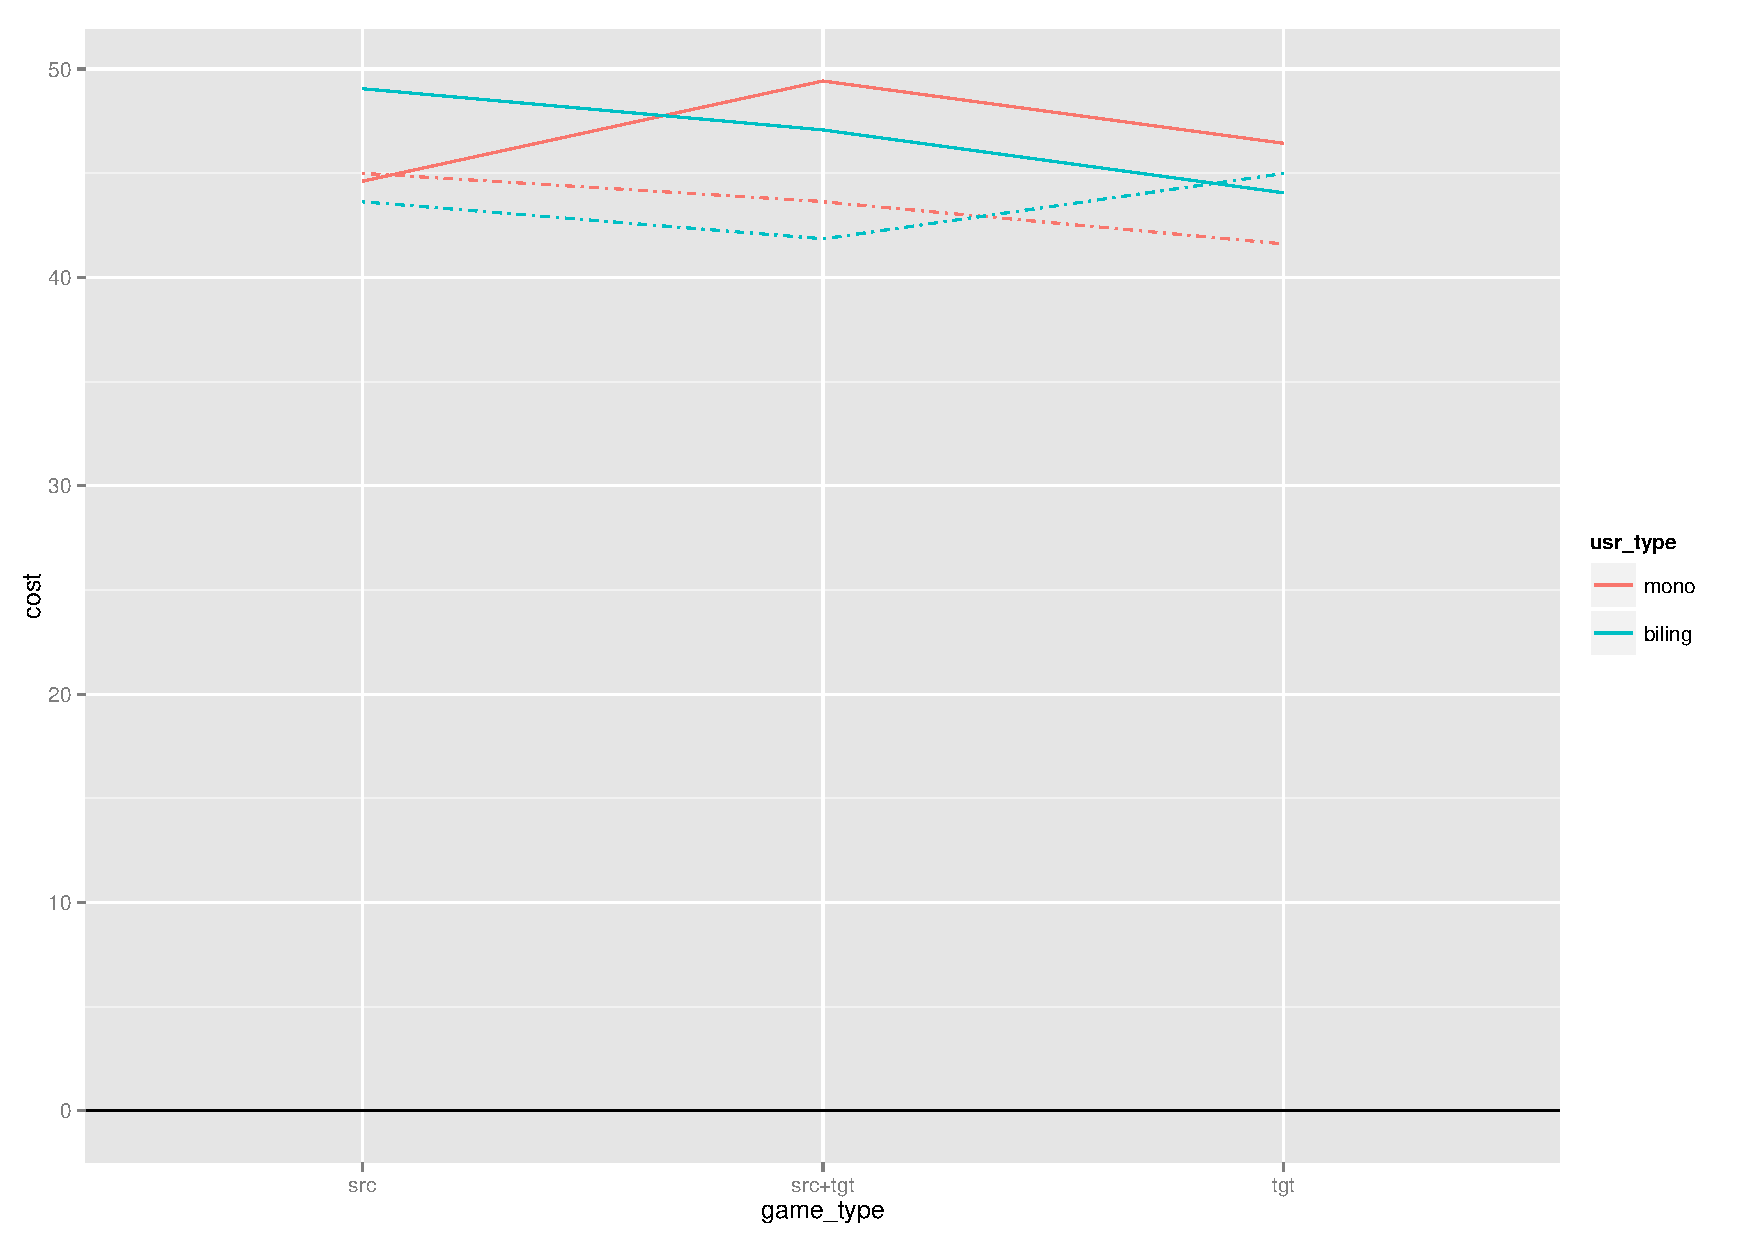
\includegraphics[scale=0.275]{data/cost_users_lm.pdf}
% \caption{Consistency of users vs humans and language model}
% \label{fig:costlm}
% \end{figure}
% \fi
\subsection{Is Bilingual Adequacy Necessary?}

Bilingual evaluators are considered to be the \emph{gold standard} for the evaluation of machine translation \cite{Dorr2011}. However, the use of monolingual evaluators has been previously advocated, since the end-users of MT are in fact monolingual \cite{Sanders2011}. The results obtained in this paper lead us to challenge the inclusion of \bil evaluators  for MT evaluation. %are really necessary for evaluating machine translation output. 
As seen in the results, \mono evaluators were slower than \bils, but they were more consistent in their evaluations. %Although in the \src \gamet they risked to evaluate only the readability of the translation (as also reported by some of our monolingual evaluators), there was no such risk in the remaining \gamets where the reference translation was provided. 
Given the open-ended nature of \bil evaluation (e.g. given a source text, they can formulate their  own set of plausible translations), we believe that the evaluations of \bils can be more subjective and prone to influence by the evaluator's background and knowledge of a specific subject.  Moreover,
 recruiting \bil evaluators can be harder and more expensive. %by the mismatch of their own mental translations with the MT output or the reference translation
We consider that consistency should be a primary goal of any evaluation task. Therefore, it seems more practical to rely only on \monos for the evaluation of machine translation. Our findings are in line with the observations in the post-editing community where \monos were more apt for the task and improved the fluency and comprehensibility of translations~\cite{mitchell2013community}. Our findings are also in partial agreement with White et al.~\shortcite{white1993evaluation} (which is not directly comparable to our work, as it does not compare monolinguals and bilinguals performing the same task), who state that less time is spent in evaluation techniques that use only target side information. 

%Our findings are in line with previous observations in the MT evaluation community where \monos seemed to perform better than \bils for a number of criteria (e.g. time) ~\cite{mitchell2013community,white1993evaluation}.

\subsection{Can Feedback Bias the Evaluation?}\label{ss:disc_feedback}
The process of evaluation can be cumbersome, especially if the evaluation sessions last for long; hence we used feedback to boost the engagement of participants throughout the evaluation process. This is a double-edged sword, as the feedback has the potential to bias the evaluators and influence their decision. %This is specially troublesome since we used scores coming from a different task (i.e. ranking) and from an automatic metric to compute feedback scores. 
\pagebreak

To rule-out any potential bias from the feedback, we investigated the effects that the progression in which the tasks were performed might have on the differences between the evaluator scores and the feedback scores. %standard deviation of the user's score with respect to the feedback scores 

If the evaluators \emph{learned} to reproduce the feedback scores, we would expect that the feedback error ($\tau_c$) would decrease as a function of time. \\
We calculated the feedback error as follows:

%Additionally, we measured the deviation with respect to the \emph{corrected} human raking scores used for \emph{feedback}, to get an idea of which type of users were \emph{closer} to the translation quality obtained with ranking. 
%We calculated the deviation $\tau$ as follows:

\begin{equation}
\tau_c^2 =   \frac{1}{N_c}\sum_{i \in T} \sum_{j\in C}(\tilde x_{ij} - f_i)^2
\end{equation}

\noindent where $f_i$ is the feedback score for translation $i$, and other variables are the same as in eq. ~\ref{eq:1}.

We fitted a linear model to the data, using the \gamet, the evaluator type and the progression (time) as predictors; and the feedback error as a response. We did not find that the progression had any significant effect ($p=0.2856$) on the feedback error.  This means that the feedback did not bias the scoring behavior of the evaluators.

\subsection{Can We do More with Eye-tracking?}
\Eye technology has proven useful in different scenarios related to translation.
%\paco{Here we give more examples of how it was used}
%So far, 
Yet, here we have only used the \eye device to measure the \emph{dwell} time an evaluator spends reading a specific portion of the screen. Nonetheless, one can think of more refined uses for this technology.

Potentially, using \eye can give us a fine-grained insight on how evaluators differentiate \emph{good} from \emph{bad} translations, making it easier to \emph{learn} the intrinsic rules of thumb that they use during the evaluation process. The applications for this are manifold. For example, by learning which type of errors (e.g. morphological, syntactic, semantic) can make a stronger impact on the reading behavior while evaluating, we could help to develop \emph{better} automatic MT evaluation metrics. Additionally, we can use gaze-data to model the evaluation score (or rank) given by an evaluator, and thus reduce the subjective score bias. This can help to alleviate the high variance found in evaluation. 

However, there are several challenges that need to be solved before moving forward in this nascent area. The most important is related to the accuracy of the \eye devices, which is a requirement to track which specific words are looked-at in the screen. 
\pagebreak

\Eye errors can be divided into two categories: variable (device-related precision) and systematic. Fortunately, the former has improved over the past years, and high-precision devices can be now acquired for only a few hundred dollars. The latter, however is more complex. Often, a loss in accuracy known as \emph{drift} is observed as time progresses, requiring frequent re-calibrations of the \eye device. \\
This can be due to evaluator movements, and other environmental factors. Reducing and eliminating drift is imperative to make progress in this area. Up to now, only heuristic approaches have been proposed \cite{mishra-carl-bhattacharyya:2012:ETNLP}, leaving plenty of room for improvement.




%\section*{Acknowledgments}
\section{Conclusion}
In this paper, we analyzed the process of MT evaluation from a \emph{glass-box} perspective, using \eye data. We contrasted two main aspects of the evaluation tasks: the background of the evaluators, and the sources of information available to them during the evaluation task.
We used time and consistency as our main criteria for comparison. 
Our results show that: 
\Ni \mono evaluators take relatively longer to evaluate translations (except when only the target language information is available, then they complete the tasks in less time), yet they are more consistent in their judgements. 
\Nii The amount of information provided to evaluators can affect their performance. We observed that when more information is available, the tasks take longer to complete, and yield less consistent results.  
%\Niii We observed that \monos behave more consistently and complete the tasks in less time when only the target language information is available.  \stephan{This last observation is included in the previous.}

%directly proportional to the total time spent on the evaluation task but is inversely proportional to the time spent to assimilate the translation itself. Evaluators’ background had an impact on the evaluation procss outcomes. Monolinguals showed more consistent and hence more reliable evaluation when contrasted with bilinguals. The ramification of the latter conclusion is important and more precisely on large evaluation campaigns where access to bilinguals might impede the process for either the availability or the cost. 

%We analyzed the orthodox human evaluation process using \eye. We looked at three aspects: evaluation time, sources of information (scenarios) and evaluator background (\emph{monolingual or bilingual}). Our results showed that \bil takes relatively less time to evaluate compared to monolinguals. The amount of information provided to evaluators is directly proportional to the total time spent on the evaluation task but is inversely proportional to the time spent to assimilate the translation itself. Evaluators’ background had an impact on the evaluation procss outcomes. Monolinguals showed more consistent and hence more reliable evaluation when contrasted with bilinguals. 

Therefore, based on our empirical results, we suggest that future evaluation campaigns be done with \mono evaluators in a \tgt \gamet. We argue that this setting can increase the consistency of results while reducing the potential costs of recruiting \bils. 
%to The ramification of the latter conclusion is important and more precisely on large evaluation campaigns where access to bilinguals might impede the process for either the availability or the cost. 

In future studies we would like to extend our explorations into using \eye to model the behavior of evaluators and to help predict reliable and unreliable translations.  In particular, we would like to explore the application of \eye in ranking scenarios. We believe that given the popularity and availability of \emph{low-cost} devices, \eye can position itself as a useful aid to reduce subjectivity in evaluation.%, making them more consistent. 

%by adding useful information that would substitute explicit score with potential biases. 
%The fixation can help to identify difficult and problematic regions of translation which could move 

\pagebreak
\bibliographystyle{acl}
\bibliography{eyetracking}

\end{document}
